\chapter{SKIP/SCROLL} 
\label{sec:scrolling}
\lstset{style=6502Style}

Scrolling is hard to do well, even when the computer's hardware provides affordances that are supposed
to make it easy. \textit{Uridium} is famous for it's silky smooth and rapid scrolling. How did it manage
to succeed where so many others of the era failed? Surely there's no avoiding the process intensive
business of moving a full screen of pixels, one at a time, to give the player the impression of effortless
movement back and forth across the surface of the enemy dreadnought? What if instead of trying to move a pixel
at a time we instead devised a method of displaying \textit{any} arbitrary position on the surface? What, if instead
of scrolling, we could \icode{skip} to any location on the playfield? Surely this would also be too much work?

Like so many other problems in computer science, we can solve this one through a process of
'divide and conquer'. First, we can treat our playfield, which is 512 characters wide, as consisting
of 16 segments numbered from 0 to 15.
\begin{figure}[H]
    \begin{adjustbox}{width=13.3cm,left}
      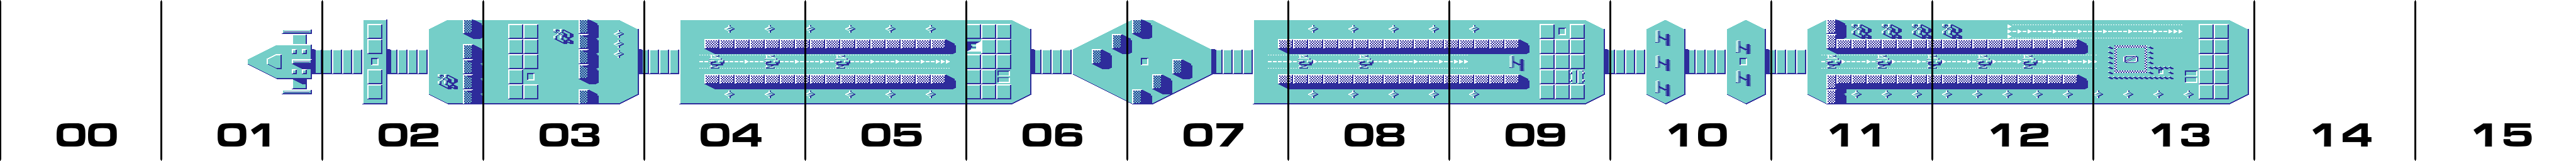
\includegraphics{src/scrolling/segments/12_scroll_segments.png}%
    \end{adjustbox}
\end{figure}
\vspace{-0.4cm}

If we have a way of keeping track which segment we are currently in we have immediately narrowed down
the problem of what to display to the player to a very narrow slice of the playfield. Let's imagine
we are currently in segment 6.

\begin{figure}[H]
    \begin{adjustbox}{width=13.3cm,left}
      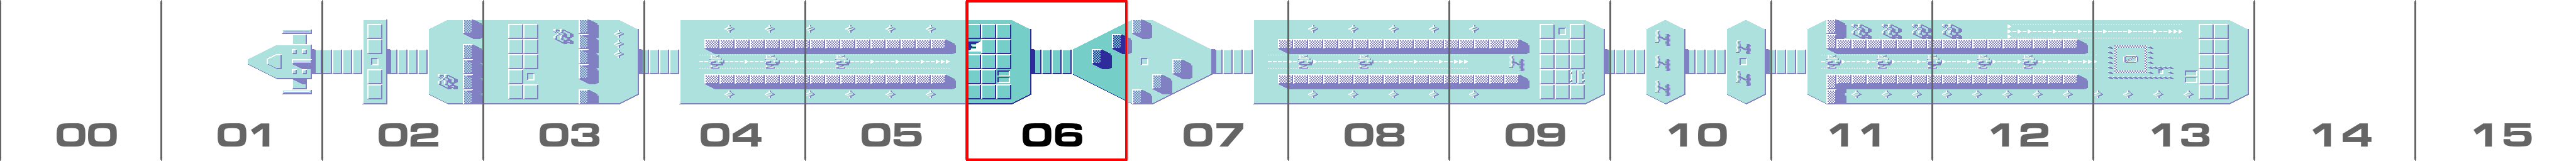
\includegraphics{src/scrolling/segments/12_scroll_segments_6_selected.png}%
    \end{adjustbox}
\end{figure}
\vspace{-0.4cm}

When we zoom in to take a closer look at this segment we begin to see that sixteen as our number
of segments is more than just an arbitrary number. Each segment is 32 characters wide and
since each character is 8 pixels wide (as illustrated by the inset in the bottom right), each segment will always be 256 (32 * 8) pixels across. 

\begin{figure}[H]
    \begin{adjustbox}{width=13.3cm,left}
      \includegraphics{src/scrolling/segment_inset.png}%
    \end{adjustbox}
\end{figure}
\vspace{-0.4cm}

So in order to keep track of our pixel position within the current
segment, we will need a second counter, one that will always tell us which exact pixel in the segment
we have scrolled and which alway be a value which will always be between \icode{0} and \icode{256}.

With two counters to keep track of our position on the playfield, one for telling us which scroll segment
we're in (which we'll call \icode{segment}) and the other for telling us which pixel in the segment (which
we'll call \icode{pixelX}), we have a mechanism for unlocking the ability to snap to any place in the map
regardless of our current position. This means that we can increment these counters by values of our choosing
and achieve accelerated movement across the field of play when we desire it.

How this might work in practice is illustrated by the dials below.

\begin{figure}[H]
    \centering
\raisebox{-0.3\totalheight}{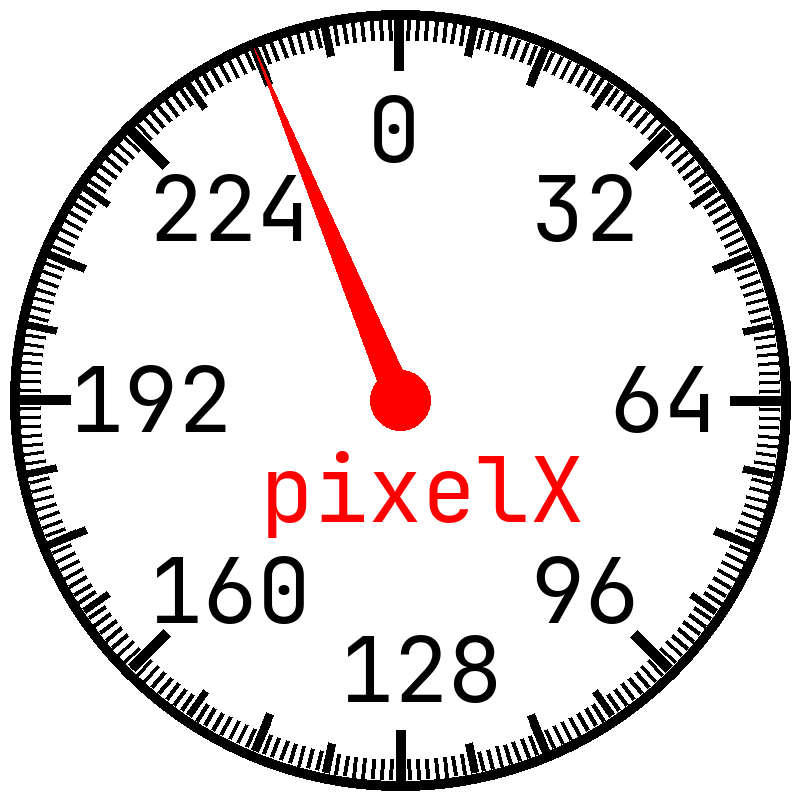
\includegraphics[height=2.2cm]{src/scrolling/dials/pixel_dial_240.png}}
\hspace{0.1cm}
\raisebox{-0.3\totalheight}{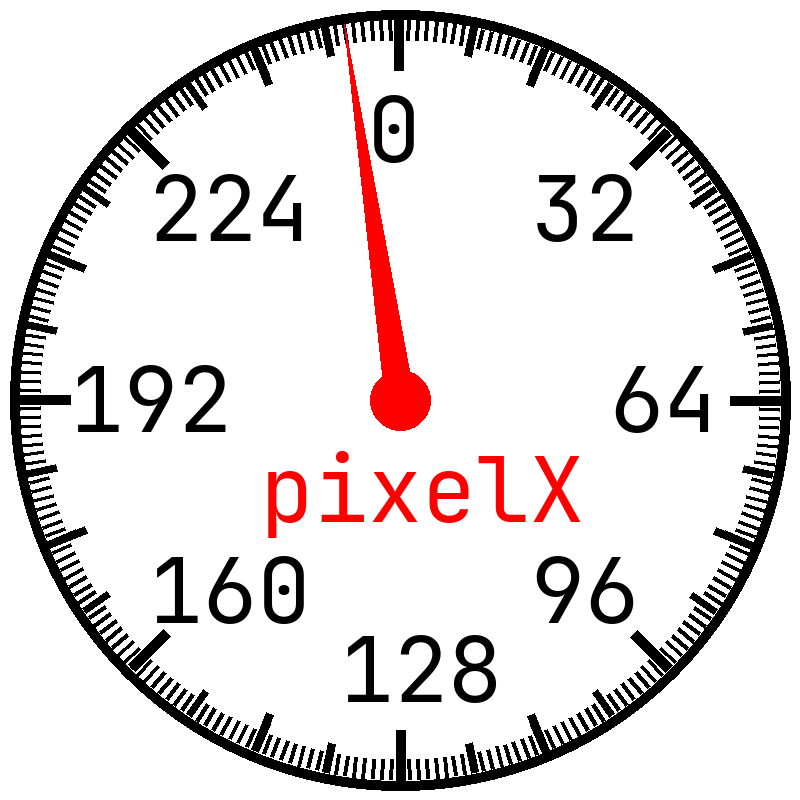
\includegraphics[height=2.2cm]{src/scrolling/dials/pixel_dial_250.png}}
\hspace{0.1cm}
\raisebox{-0.3\totalheight}{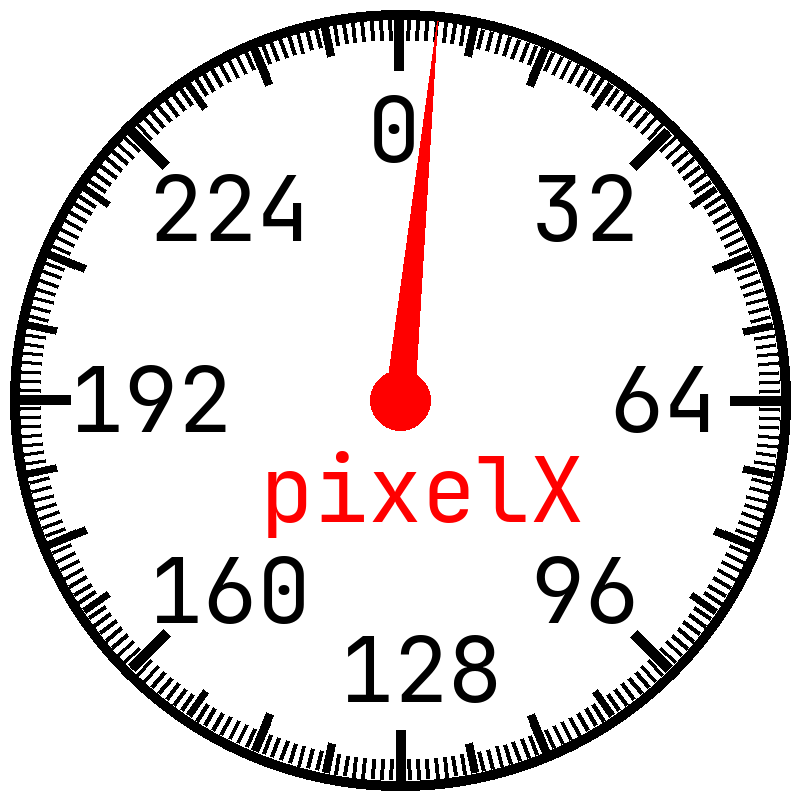
\includegraphics[height=2.2cm]{src/scrolling/dials/pixel_dial_4.png}}
\hspace{0.1cm}
\raisebox{-0.3\totalheight}{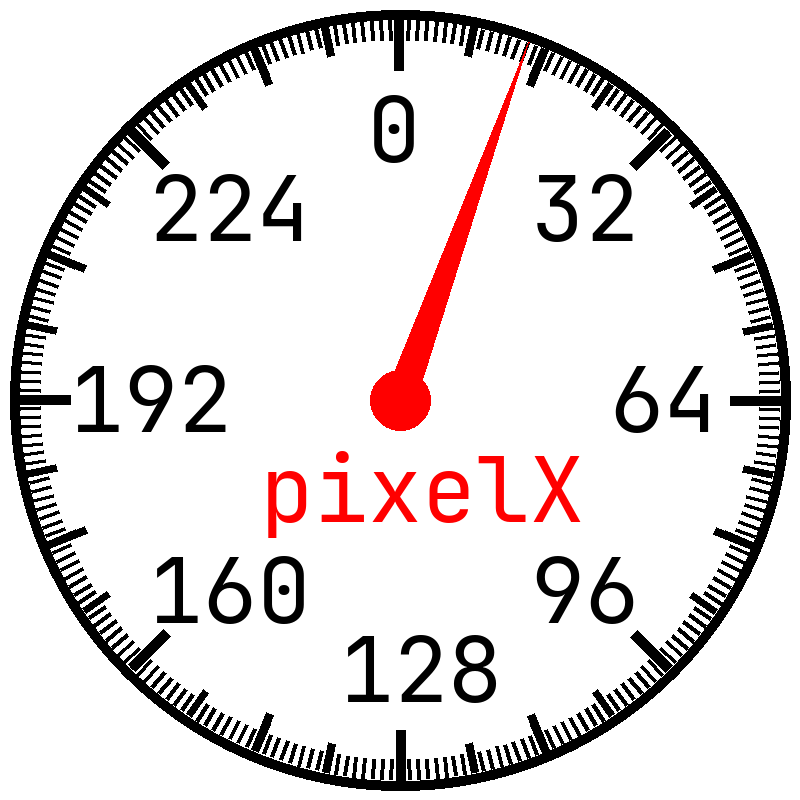
\includegraphics[height=2.2cm]{src/scrolling/dials/pixel_dial_14.png}}
\hspace{0.1cm}
\raisebox{-0.3\totalheight}{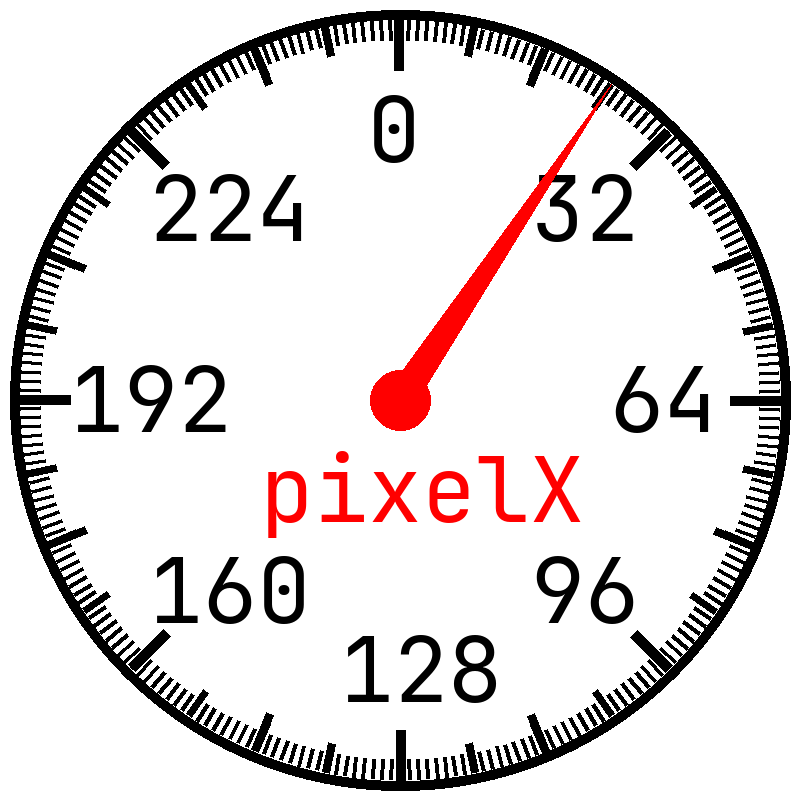
\includegraphics[height=2.2cm]{src/scrolling/dials/pixel_dial_24.png}}
\end{figure}
\vspace{-0.4cm}
\begin{figure}[H]
    \centering
\raisebox{-0.3\totalheight}{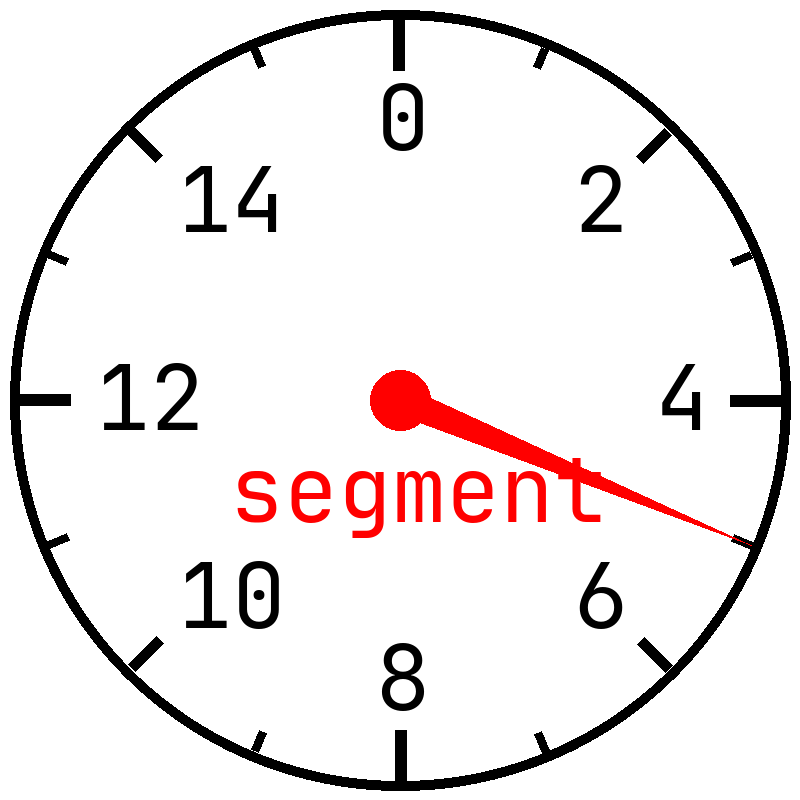
\includegraphics[height=2.2cm]{src/scrolling/dials/segment_dial_5.png}}
\hspace{0.1cm}
\raisebox{-0.3\totalheight}{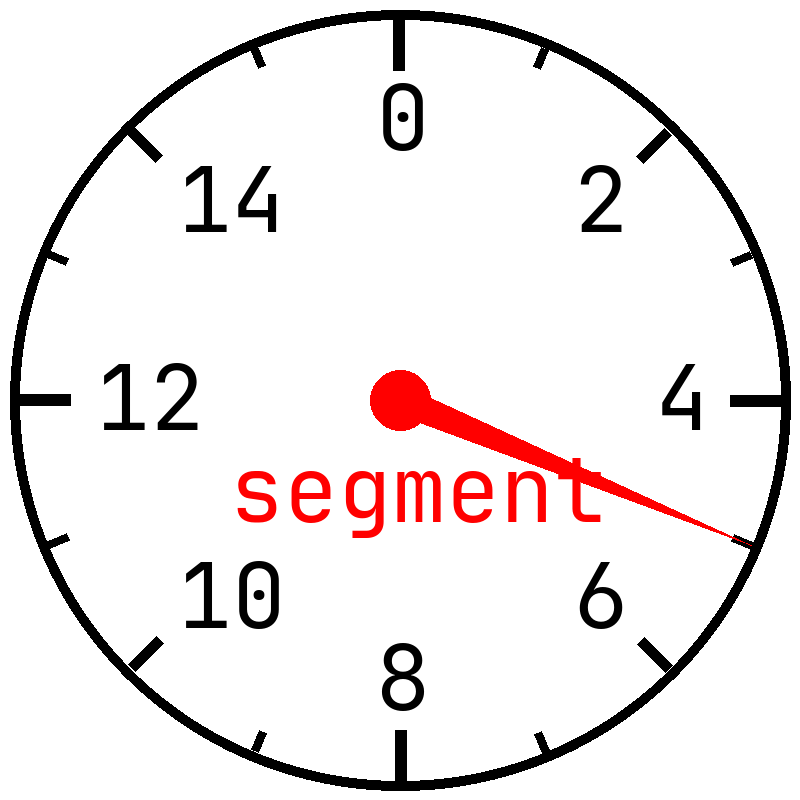
\includegraphics[height=2.2cm]{src/scrolling/dials/segment_dial_5.png}}
\hspace{0.1cm}
\raisebox{-0.3\totalheight}{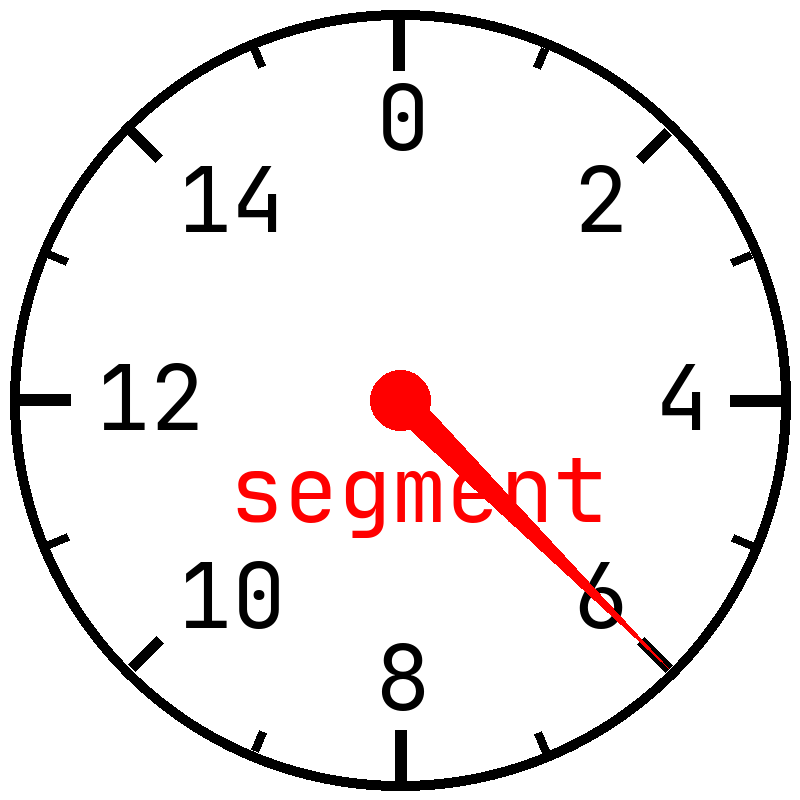
\includegraphics[height=2.2cm]{src/scrolling/dials/segment_dial_6.png}}
\hspace{0.1cm}
\raisebox{-0.3\totalheight}{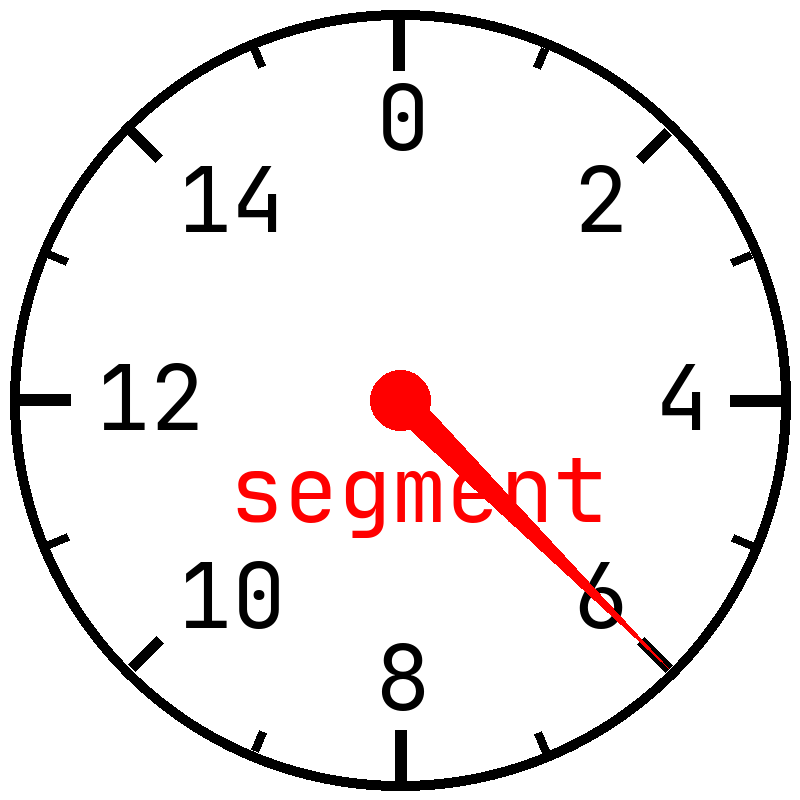
\includegraphics[height=2.2cm]{src/scrolling/dials/segment_dial_6.png}}
\hspace{0.1cm}
\raisebox{-0.3\totalheight}{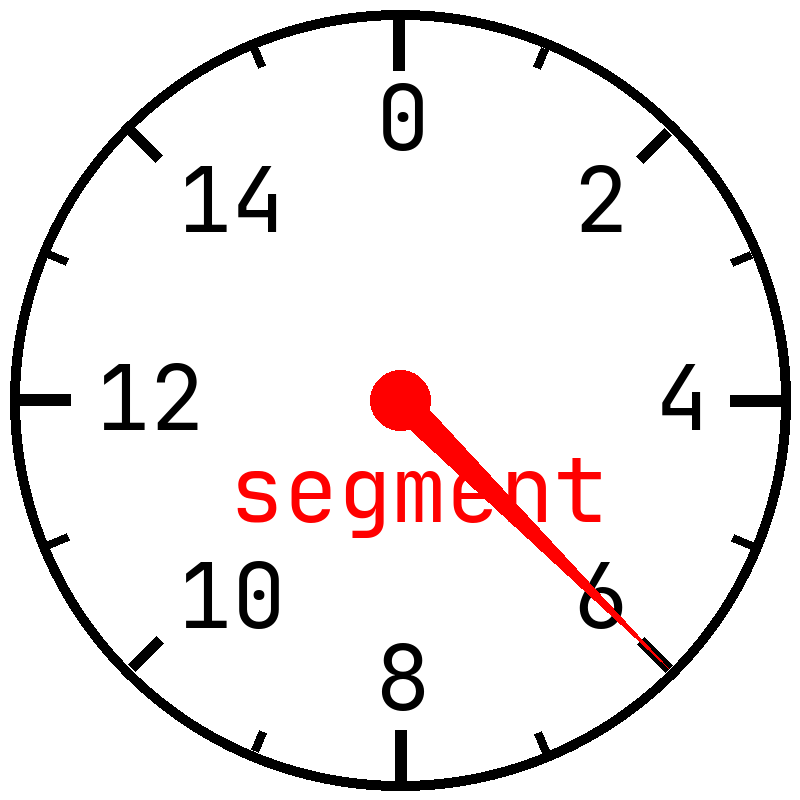
\includegraphics[height=2.2cm]{src/scrolling/dials/segment_dial_6.png}}
\end{figure}
\vspace{-0.4cm}

Here we are currently in \icode{segment} 5 and incrementing our position within the segment, \icode{pixelX},
by 10 each time. On the third increment we pass around the top of the clock and restart at zero. So an increment
of 10 from 250 brings us past 255, through 0 and up to 4. Crucially, when this happens the value for \icode{segment} is incremented
from 5 to 6. So an increment of 10 has moved us from pixel position 250 in segment 5:

\begin{figure}[H]
    \begin{adjustbox}{width=13.3cm,left}
      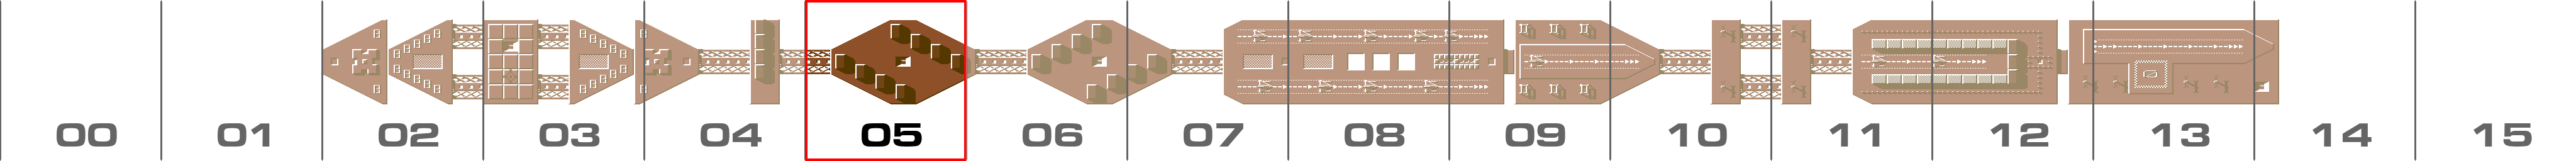
\includegraphics{src/scrolling/segments/11_scroll_segments_5_selected.png}%
    \end{adjustbox}
\end{figure}
\vspace{-0.4cm}

to position 4 in segment 6:

\begin{figure}[H]
    \begin{adjustbox}{width=13.3cm,left}
      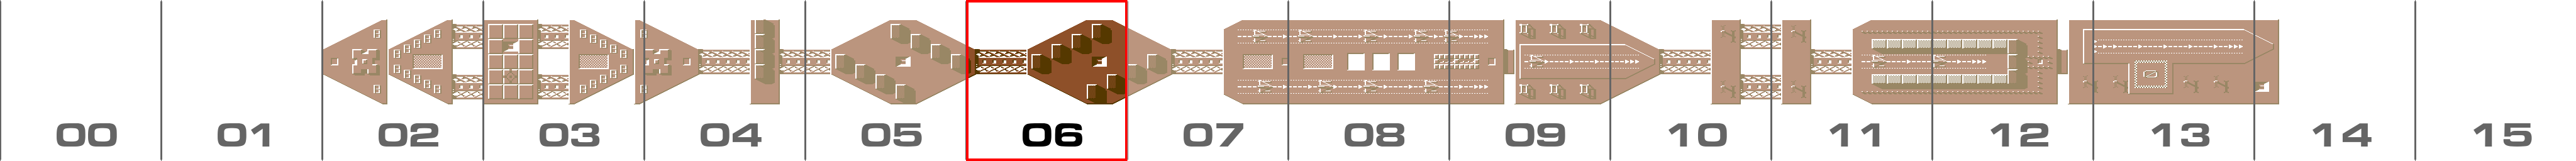
\includegraphics{src/scrolling/segments/11_scroll_segments_6_selected.png}%
    \end{adjustbox}
\end{figure}
\vspace{-0.4cm}

This lockstep scheme applies in the other direction too. In the example below, we are moving in increments of 24
from right to left, so the dials are moving in the opposite direction.

\begin{figure}[H]
    \centering
\raisebox{-0.3\totalheight}{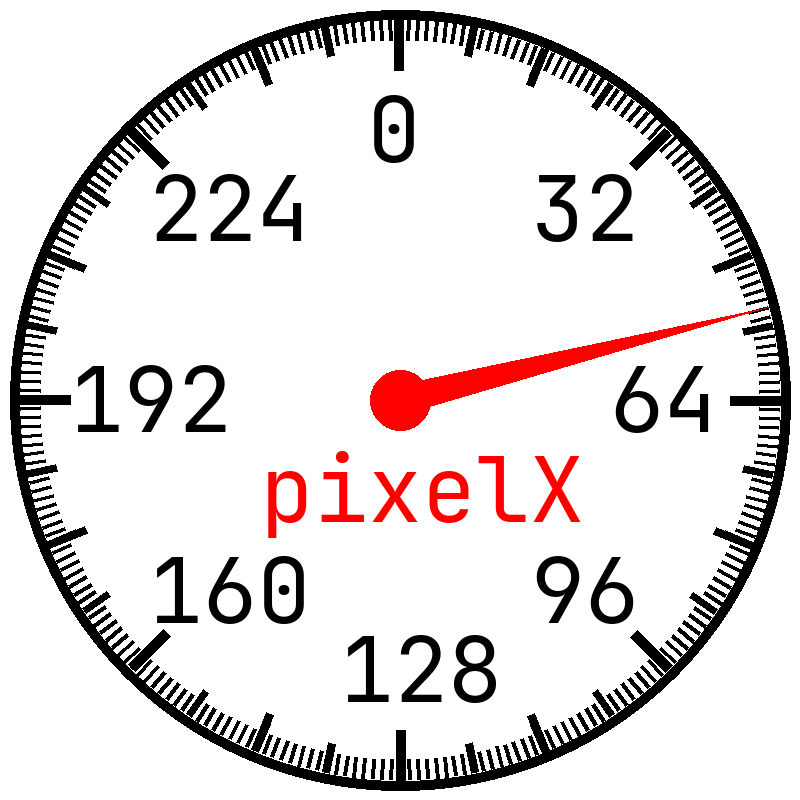
\includegraphics[height=2.2cm]{src/scrolling/dials/pixel_dial_54.png}}
\hspace{0.1cm}
\raisebox{-0.3\totalheight}{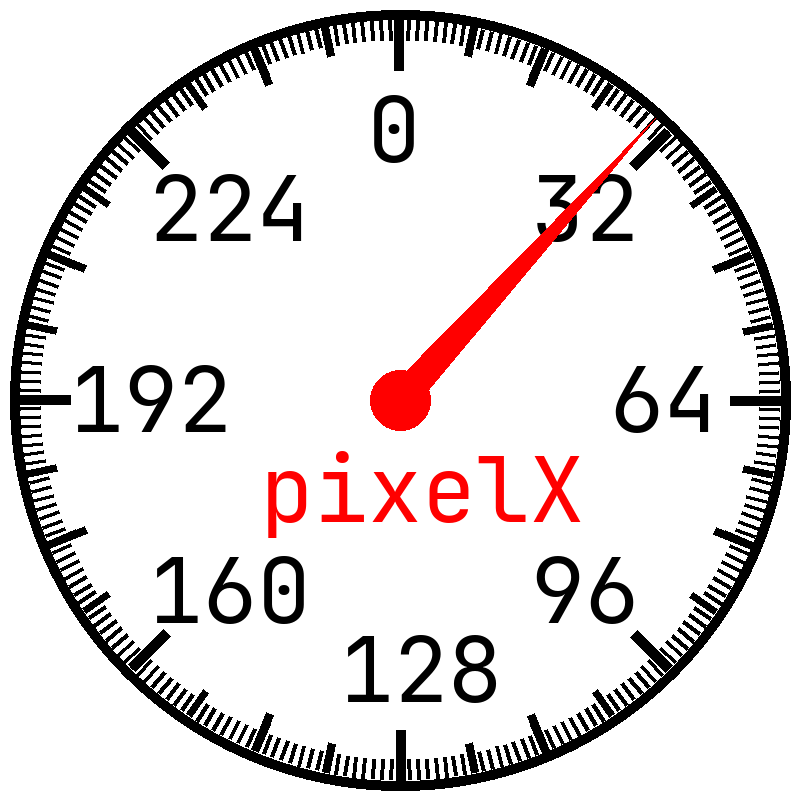
\includegraphics[height=2.2cm]{src/scrolling/dials/pixel_dial_30.png}}
\hspace{0.1cm}
\raisebox{-0.3\totalheight}{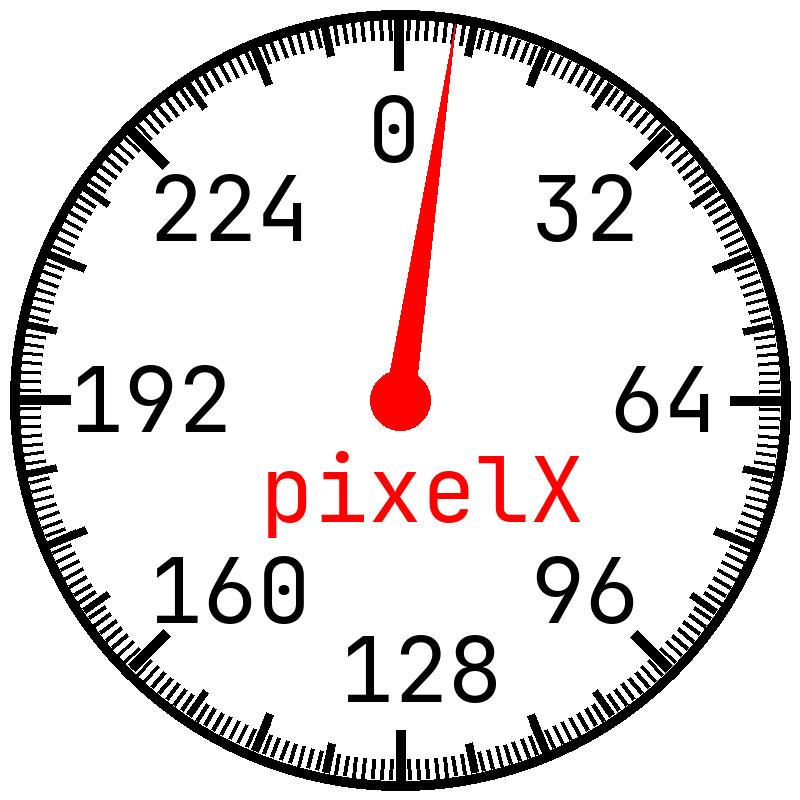
\includegraphics[height=2.2cm]{src/scrolling/dials/pixel_dial_6.png}}
\hspace{0.1cm}
\raisebox{-0.3\totalheight}{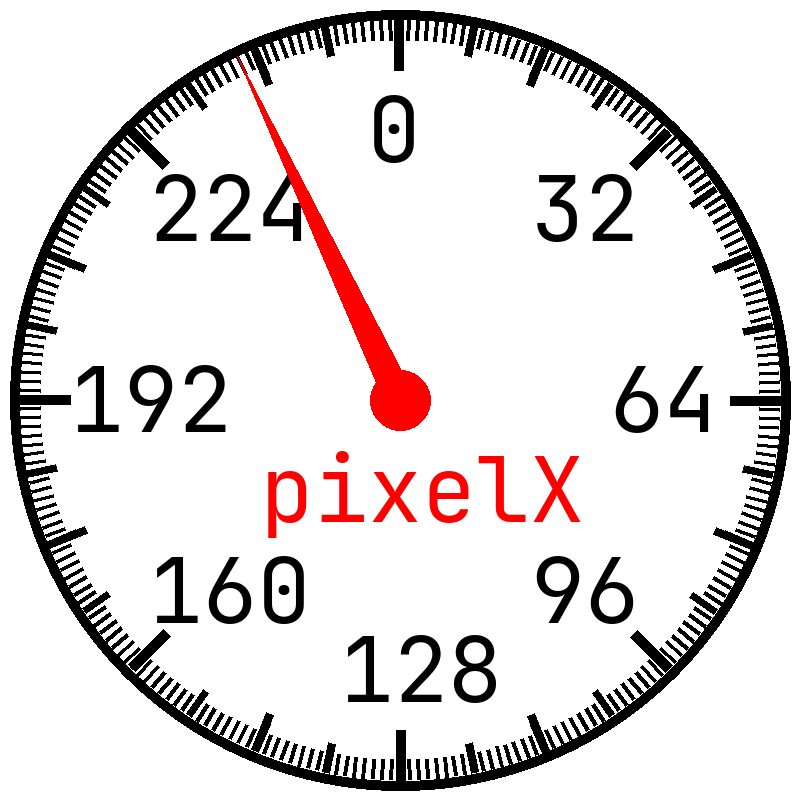
\includegraphics[height=2.2cm]{src/scrolling/dials/pixel_dial_238.png}}
\hspace{0.1cm}
\raisebox{-0.3\totalheight}{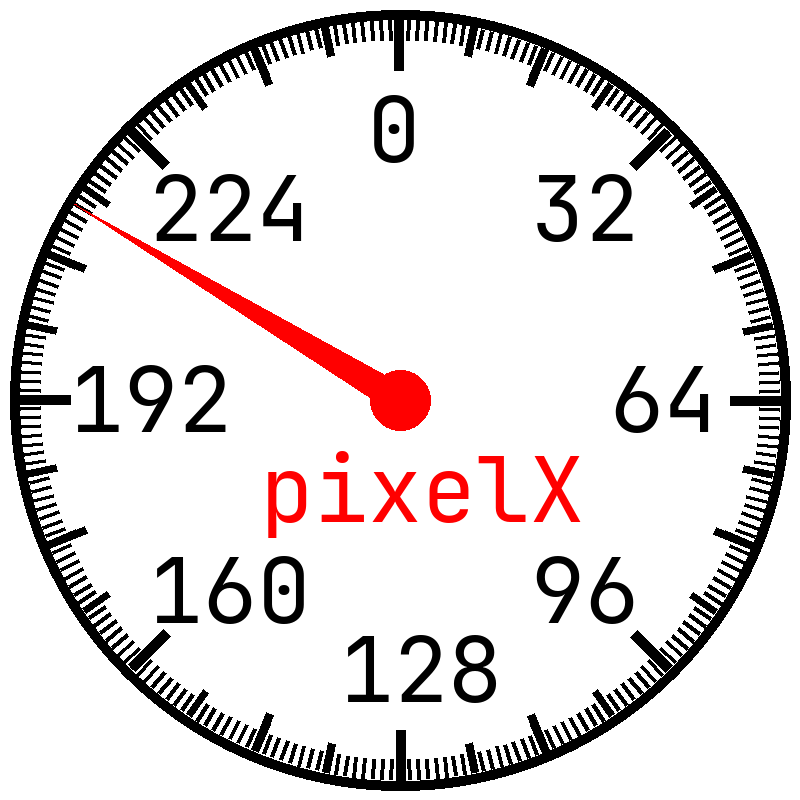
\includegraphics[height=2.2cm]{src/scrolling/dials/pixel_dial_214.png}}
\end{figure}
\vspace{-0.4cm}
\begin{figure}[H]
    \centering
\raisebox{-0.3\totalheight}{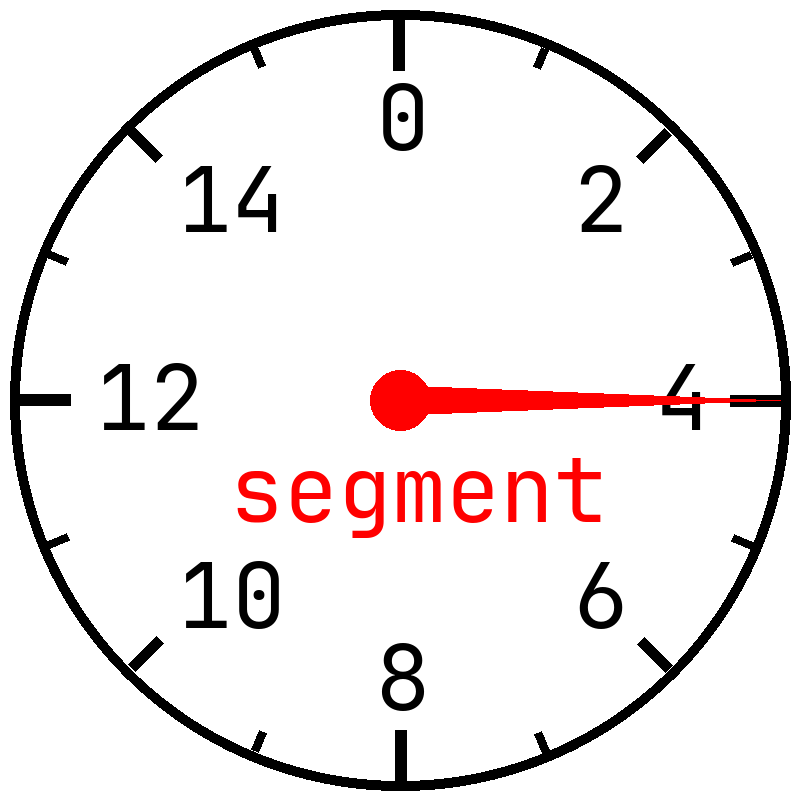
\includegraphics[height=2.2cm]{src/scrolling/dials/segment_dial_4.png}}
\hspace{0.1cm}
\raisebox{-0.3\totalheight}{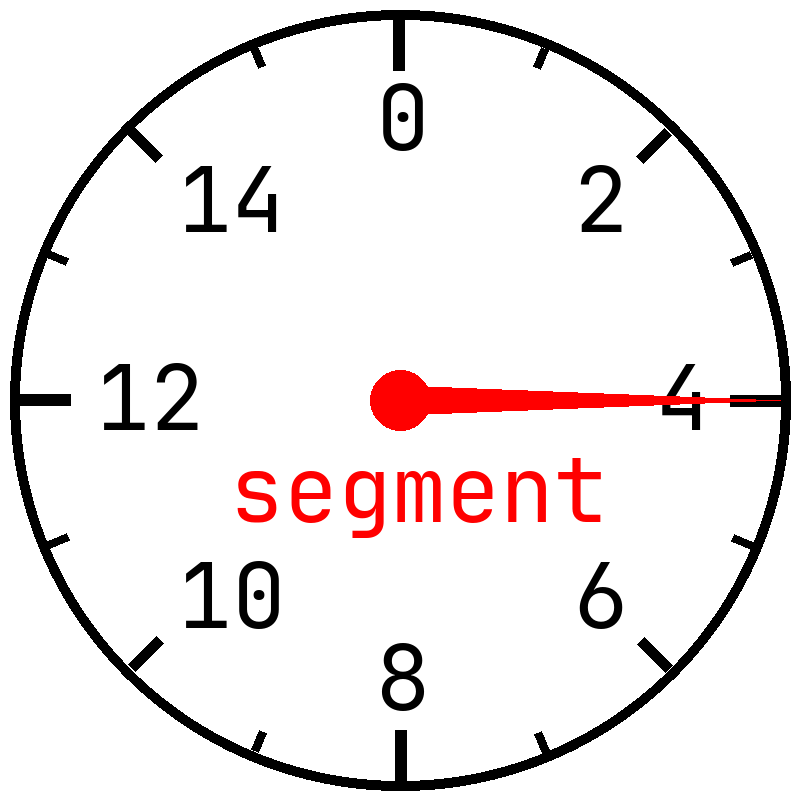
\includegraphics[height=2.2cm]{src/scrolling/dials/segment_dial_4.png}}
\hspace{0.1cm}
\raisebox{-0.3\totalheight}{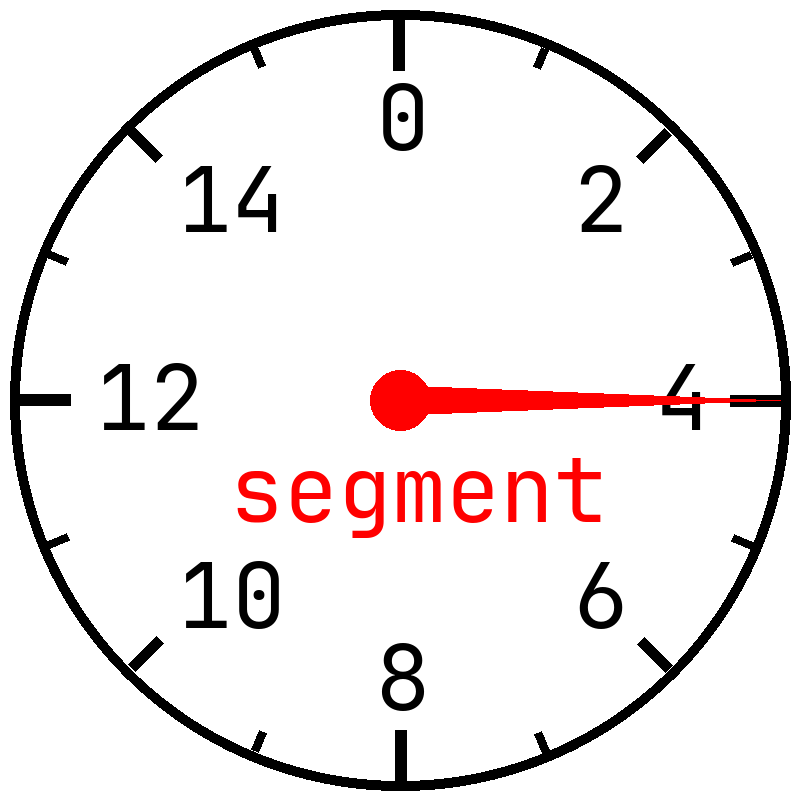
\includegraphics[height=2.2cm]{src/scrolling/dials/segment_dial_4.png}}
\hspace{0.1cm}
\raisebox{-0.3\totalheight}{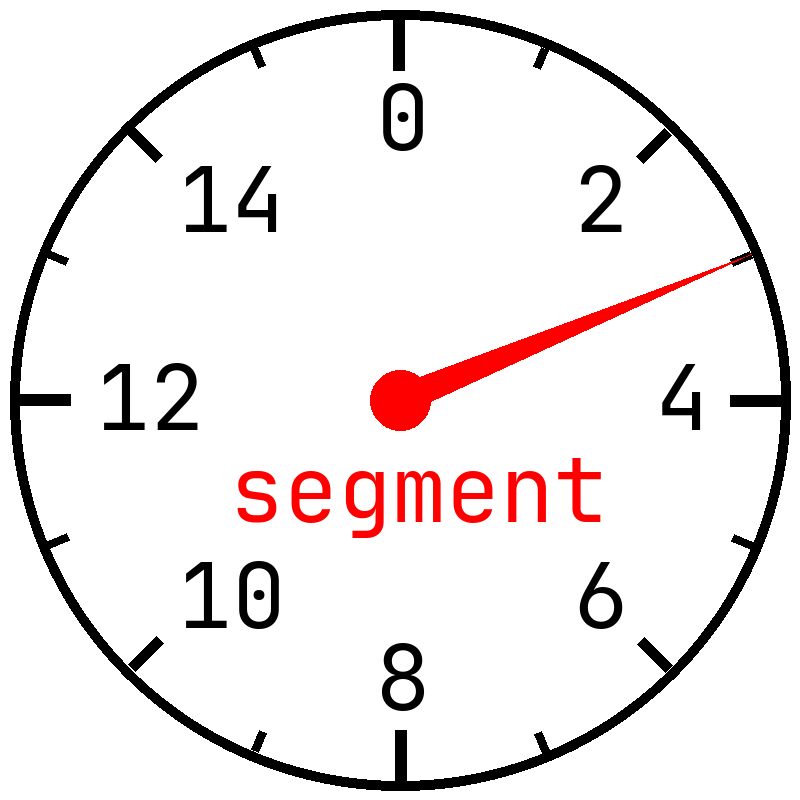
\includegraphics[height=2.2cm]{src/scrolling/dials/segment_dial_3.png}}
\hspace{0.1cm}
\raisebox{-0.3\totalheight}{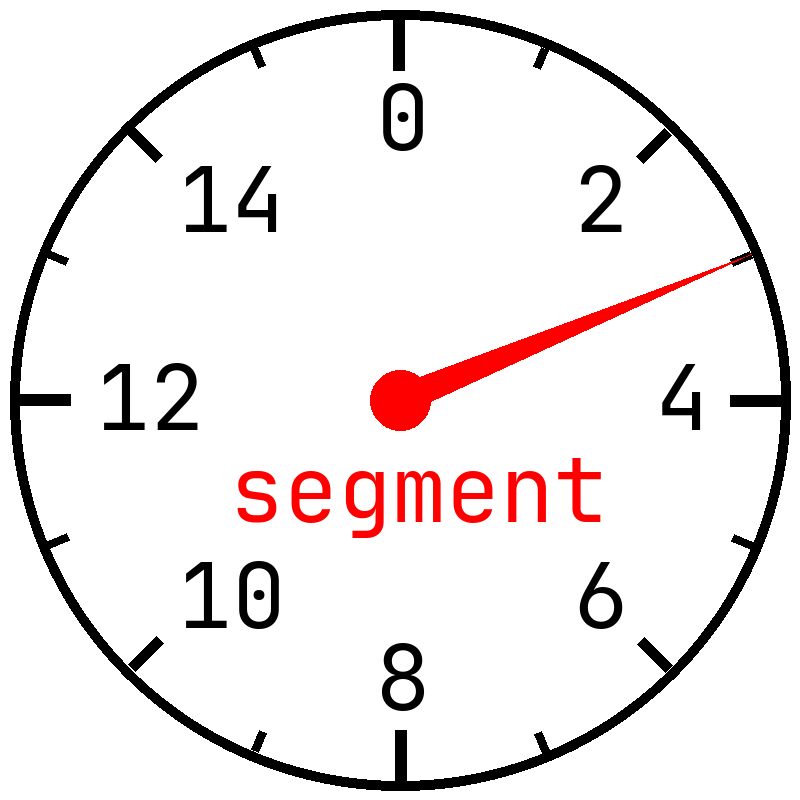
\includegraphics[height=2.2cm]{src/scrolling/dials/segment_dial_3.png}}
\end{figure}
\vspace{-0.4cm}

In this example we are starting in \icode{segment} 4 at position 54 within the segment:
\begin{figure}[H]
    \begin{adjustbox}{width=13.3cm,left}
      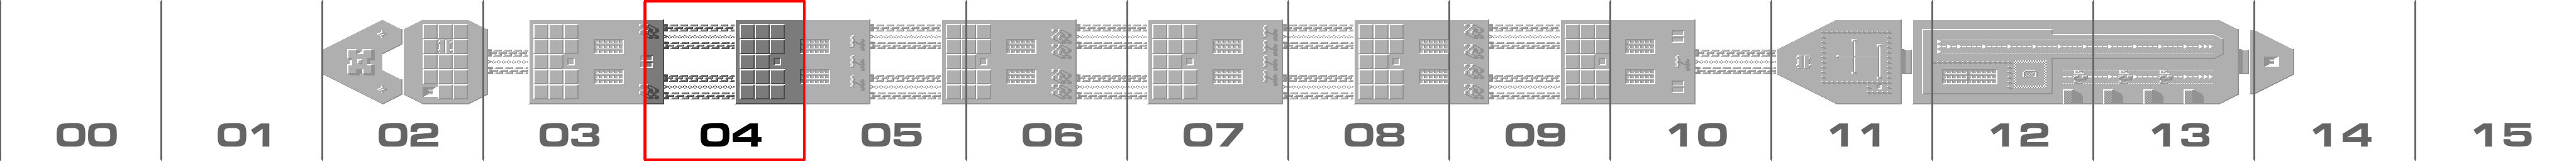
\includegraphics{src/scrolling/segments/10_scroll_segments_4_selected.png}%
    \end{adjustbox}
\end{figure}
\vspace{-0.4cm}

Our first three decrements of \icode{pixelX} have no effect on our segment position. But succesively
decrementing our \icode{pixelX} value until it wraps around past zero eventually also decrements
our \icode{segment} position by 1, moving us into \icode{segment} 3:
\begin{figure}[H]
    \begin{adjustbox}{width=13.3cm,left}
      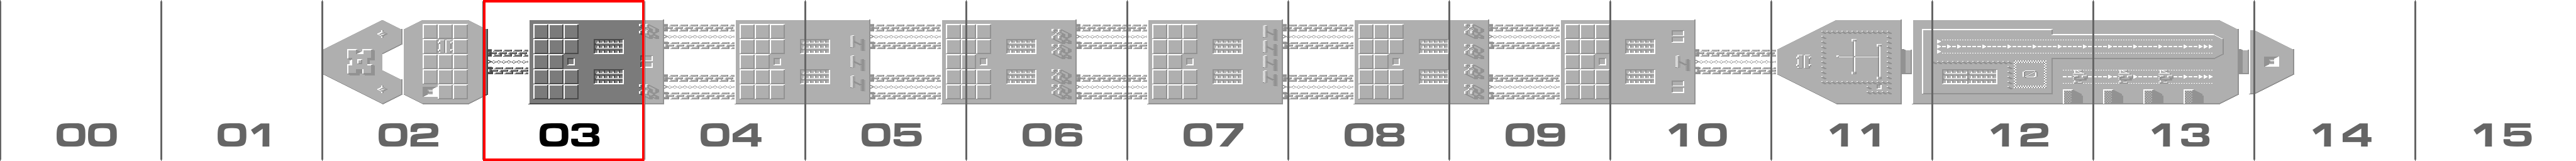
\includegraphics{src/scrolling/segments/10_scroll_segments_3_selected.png}%
    \end{adjustbox}
\end{figure}
\vspace{-0.4cm}

When we apply \icode{pixelX}, which now has a value of 214 according to our dials, we end up displaying
the screen at the following position. Notice how the position being calculated by the dials is the leftmost
position of the frame. Although our calculation position is in segment 3, the majority of the screen real estate
is occupied by segment 4:

\begin{figure}[H]
    \begin{adjustbox}{width=13.3cm,center}
      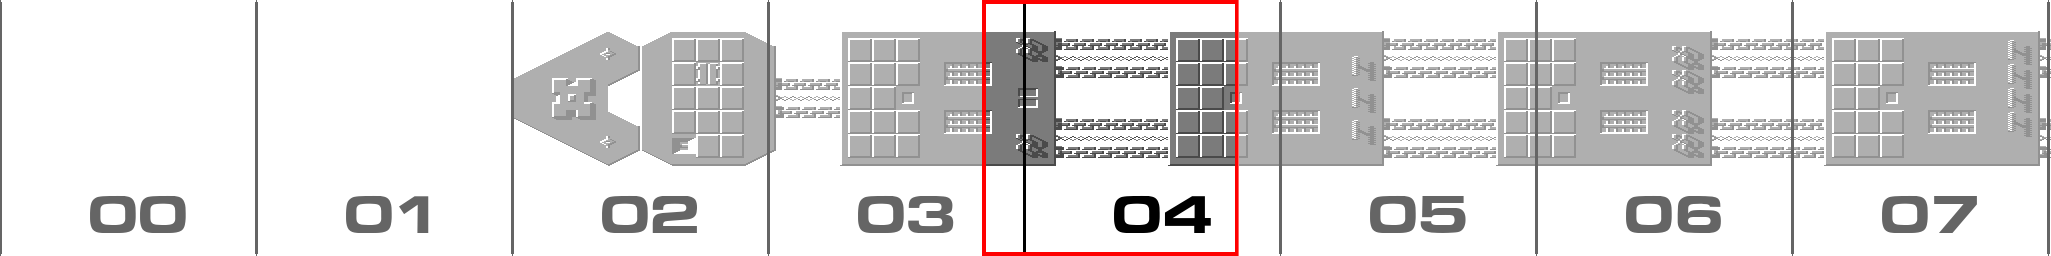
\includegraphics{src/scrolling/segments/10_scroll_segments_3_selected_214_clip.png}%
    \end{adjustbox}
\end{figure}
\vspace{-0.4cm}

The implementation of this lockstep, or gear-like, mechanism for incrementing and decrementing
our \icode{pixelX} and \icode{segment} is the relatively compact code contained in the
routine \icode{UpdateSegmentAndPixelX} given opposite.


\begin{wrapfigure}[5]{r}{3cm} % <==========================================
    \vspace{-0.4cm}
    \begin{adjustbox}{width=3cm,left}
      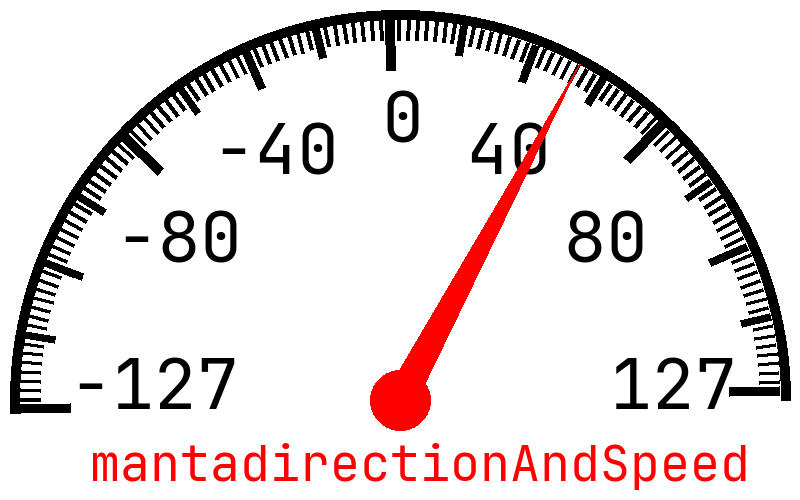
\includegraphics{src/scrolling/mantaDirectionAndSpeed.png}%
    \end{adjustbox}
\end{wrapfigure}
You'll notice that the operator used to move the dials is a variable called \icode{manta\-Direction\-AndSpeed}.
This parameter not only tells us the rate at which the manta is moving but the direction in which it is moving,
whether left or right. Like \icode{pixelX}, it has 256 possible values but in this case we treat any value over 127
as though it is negative, so it's actual range is from -127 to 127. Thus, any value between 0 and 127 is treated as the
player's velocity in a leftward direction while any value between -127 and 0 is treated as their velocity in the rightward
direction. 

Using negative values to move right and positive values to move left is counterintuitive, but it is part of the trick
that the routine achieves is to use \icode{mantaDirectionAndSpeed} to update \icode{pixelX} and detect when the dial
has moved past zero and increment or decrement \icode{segment} when required. This relies on the behaviour of setting
the 6502 processor's \textit{carry bit} when applying \icode{mantaDirectionAndSpeed} to our \icode{pixelX} value. This
\textit{carry bit} is the latch that triggers our value for \icode{segment} to move up and down as appropriate.

Up to now we haven't worried too much about how we can turn \icode{pixelX}, or \icode{segment}, into memory addresses
that give us the exact position on the playfield that they refer to. We do however get a first inkling that something
of this nature is required 
\begin{wrapfigure}[6]{l}{4.3cm} % <==========================================
    \vspace{-0.4cm}
    \begin{adjustbox}{width=4.3cm,right}
      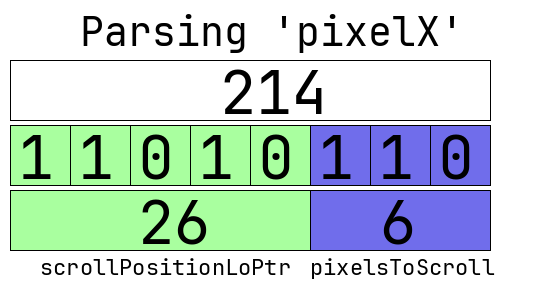
\includegraphics{src/scrolling/pixelX.png}%
    \end{adjustbox}
\end{wrapfigure}
when we see what is happening in the \icode{UpdatePixelsToScroll} paragraph opposite. We
extract the last three bits (in purple) and store them in \icode{pixelsToScroll}. This value, which will be between
0 and 8, is what gives us the pixel-level precision for the scroll.

\vspace*{\fill}
\begin{lstlisting}
;---------------------------------------------------------------------
; This routine uses mantaDirectionAndSpeed to update pixelX and
; segment. It then uses the updated pixelX value to update
; pixelsToScroll.
;---------------------------------------------------------------------
UpdateSegmentAndPixelX
  ; mantaDirectionAndSpeed is a value between -127 and 127. A negative
  ; value tells us to move right by the number of pixels, a positive
  ; value tells us to move left.
  LDA mantaDirectionAndSpeed  ; Load direction & speed to A.
  BEQ UpdatePixelsToScroll    ; If 0, no scrolling.
  BPL ScrollLeft              ; If positive, move left.

ScrollRight
  ; Set the scroll position with a precision at the character level.
  LDA pixelX                  ; Load current pixel-level movement.
  SEC                         ; Set carry.
  SBC mantaDirectionAndSpeed  ; Add the current speed value.
  STA pixelX                  ; Store it as the number of pixels to move.

  ; Update the current scroll segment.
  ; This will increment 'segment' and move to next segment if carry bit
  ; is set. It will stay on the current segment if carry bit is not set.
  LDA segment                 ; Load the current segment value.
  SBC #-1                     ; Subtract -1.
  STA segment                 ; Update segment with the result.

  ; Set the scroll position with a precision of 8 bits within the character
  ; by taking the last three bits of pixelX.
UpdatePixelsToScroll
  LDA #$08                    ; Load 8 to A.
  SEC                         ; Set the carry bit.
  SBC pixelX                  ; Subtract pixelX.
  AND #$07                    ; Take the last 3 bits only..
  STA pixelsToScroll          ; .. and store in pixelsToScroll.
  RTS                         ; We're done - return.

ScrollLeft
  ; Set the scroll position with a precision at the character level.
  LDA pixelX                  ; Load current pixel-level movement.
  SEC                         ; Set carry.
  SBC mantaDirectionAndSpeed  ; Add the current speed value.
  STA pixelX                  ; Store it as the number of pixels to move.

  ; Update the current scroll segment.
  ; This will decrement 'segment' and move to previous segment if carry bit
  ; is not set. It will stay on current segment if carry bit is set.
  LDA segment                 ; Load the current segment value.
  SBC #0                      ; Subtract carry bit only.
  STA segment                 ; Update segment with the result.

  JMP UpdatePixelsToScroll    ; Updated pixelsToScroll and return.
\end{lstlisting}
\vspace*{\fill}
\clearpage
The remaining bits (in green) are what we will use
to calculate which of the 32 characters in the \icode{segment} we are at, our memory
position within the scroll \icode{segment}. The trick will be
turning this number, such as '26', into an offset in the \icode{segment} address.

Before we see how we do this, let's take stock of the mapping we want to perform. With our playfield
split into 16 segments we want to be able to take a \icode{segment} value and map it to memory
addresses within the playfield as follows:
\begin{figure}[H]
    \begin{adjustbox}{width=13.3cm,center}
      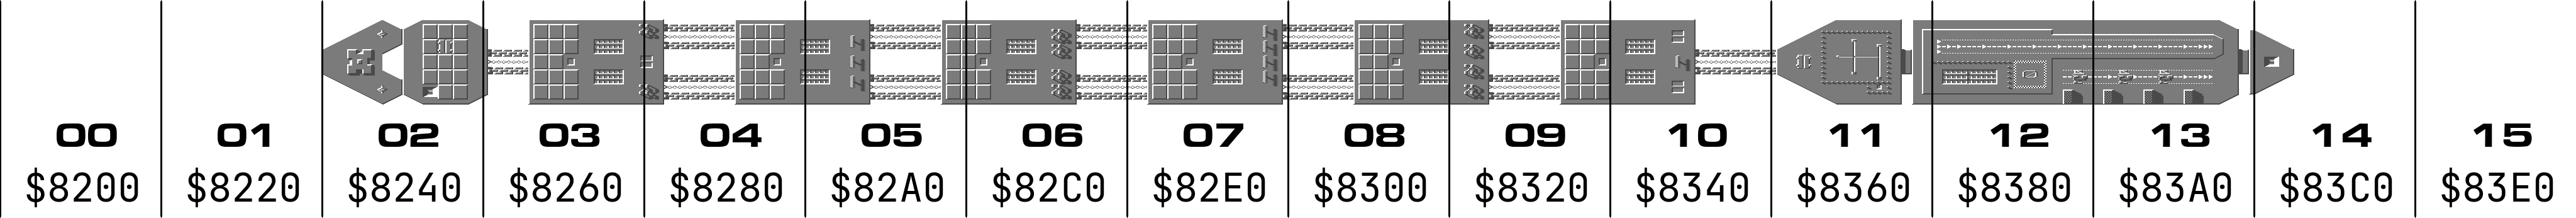
\includegraphics{src/scrolling/segments/10_scroll_segments_addresses.png}%
    \end{adjustbox}
\end{figure}
\vspace{-0.4cm}

We can think of each address above as representing the memory address for the top left of each \icode{segment}.
We then need to take the top 5 'green' bits of \icode{pixelX} and convert that into a memory position within the segment.
So starting with the simplest version of this problem, imagine we have a \icode{segment} value of \icode{\$04} and a \icode{pixelX} value of 0.
This means we will want to select the start of segment 4 as our scroll position:

\begin{figure}[H]
    \begin{adjustbox}{width=13.3cm,left}
      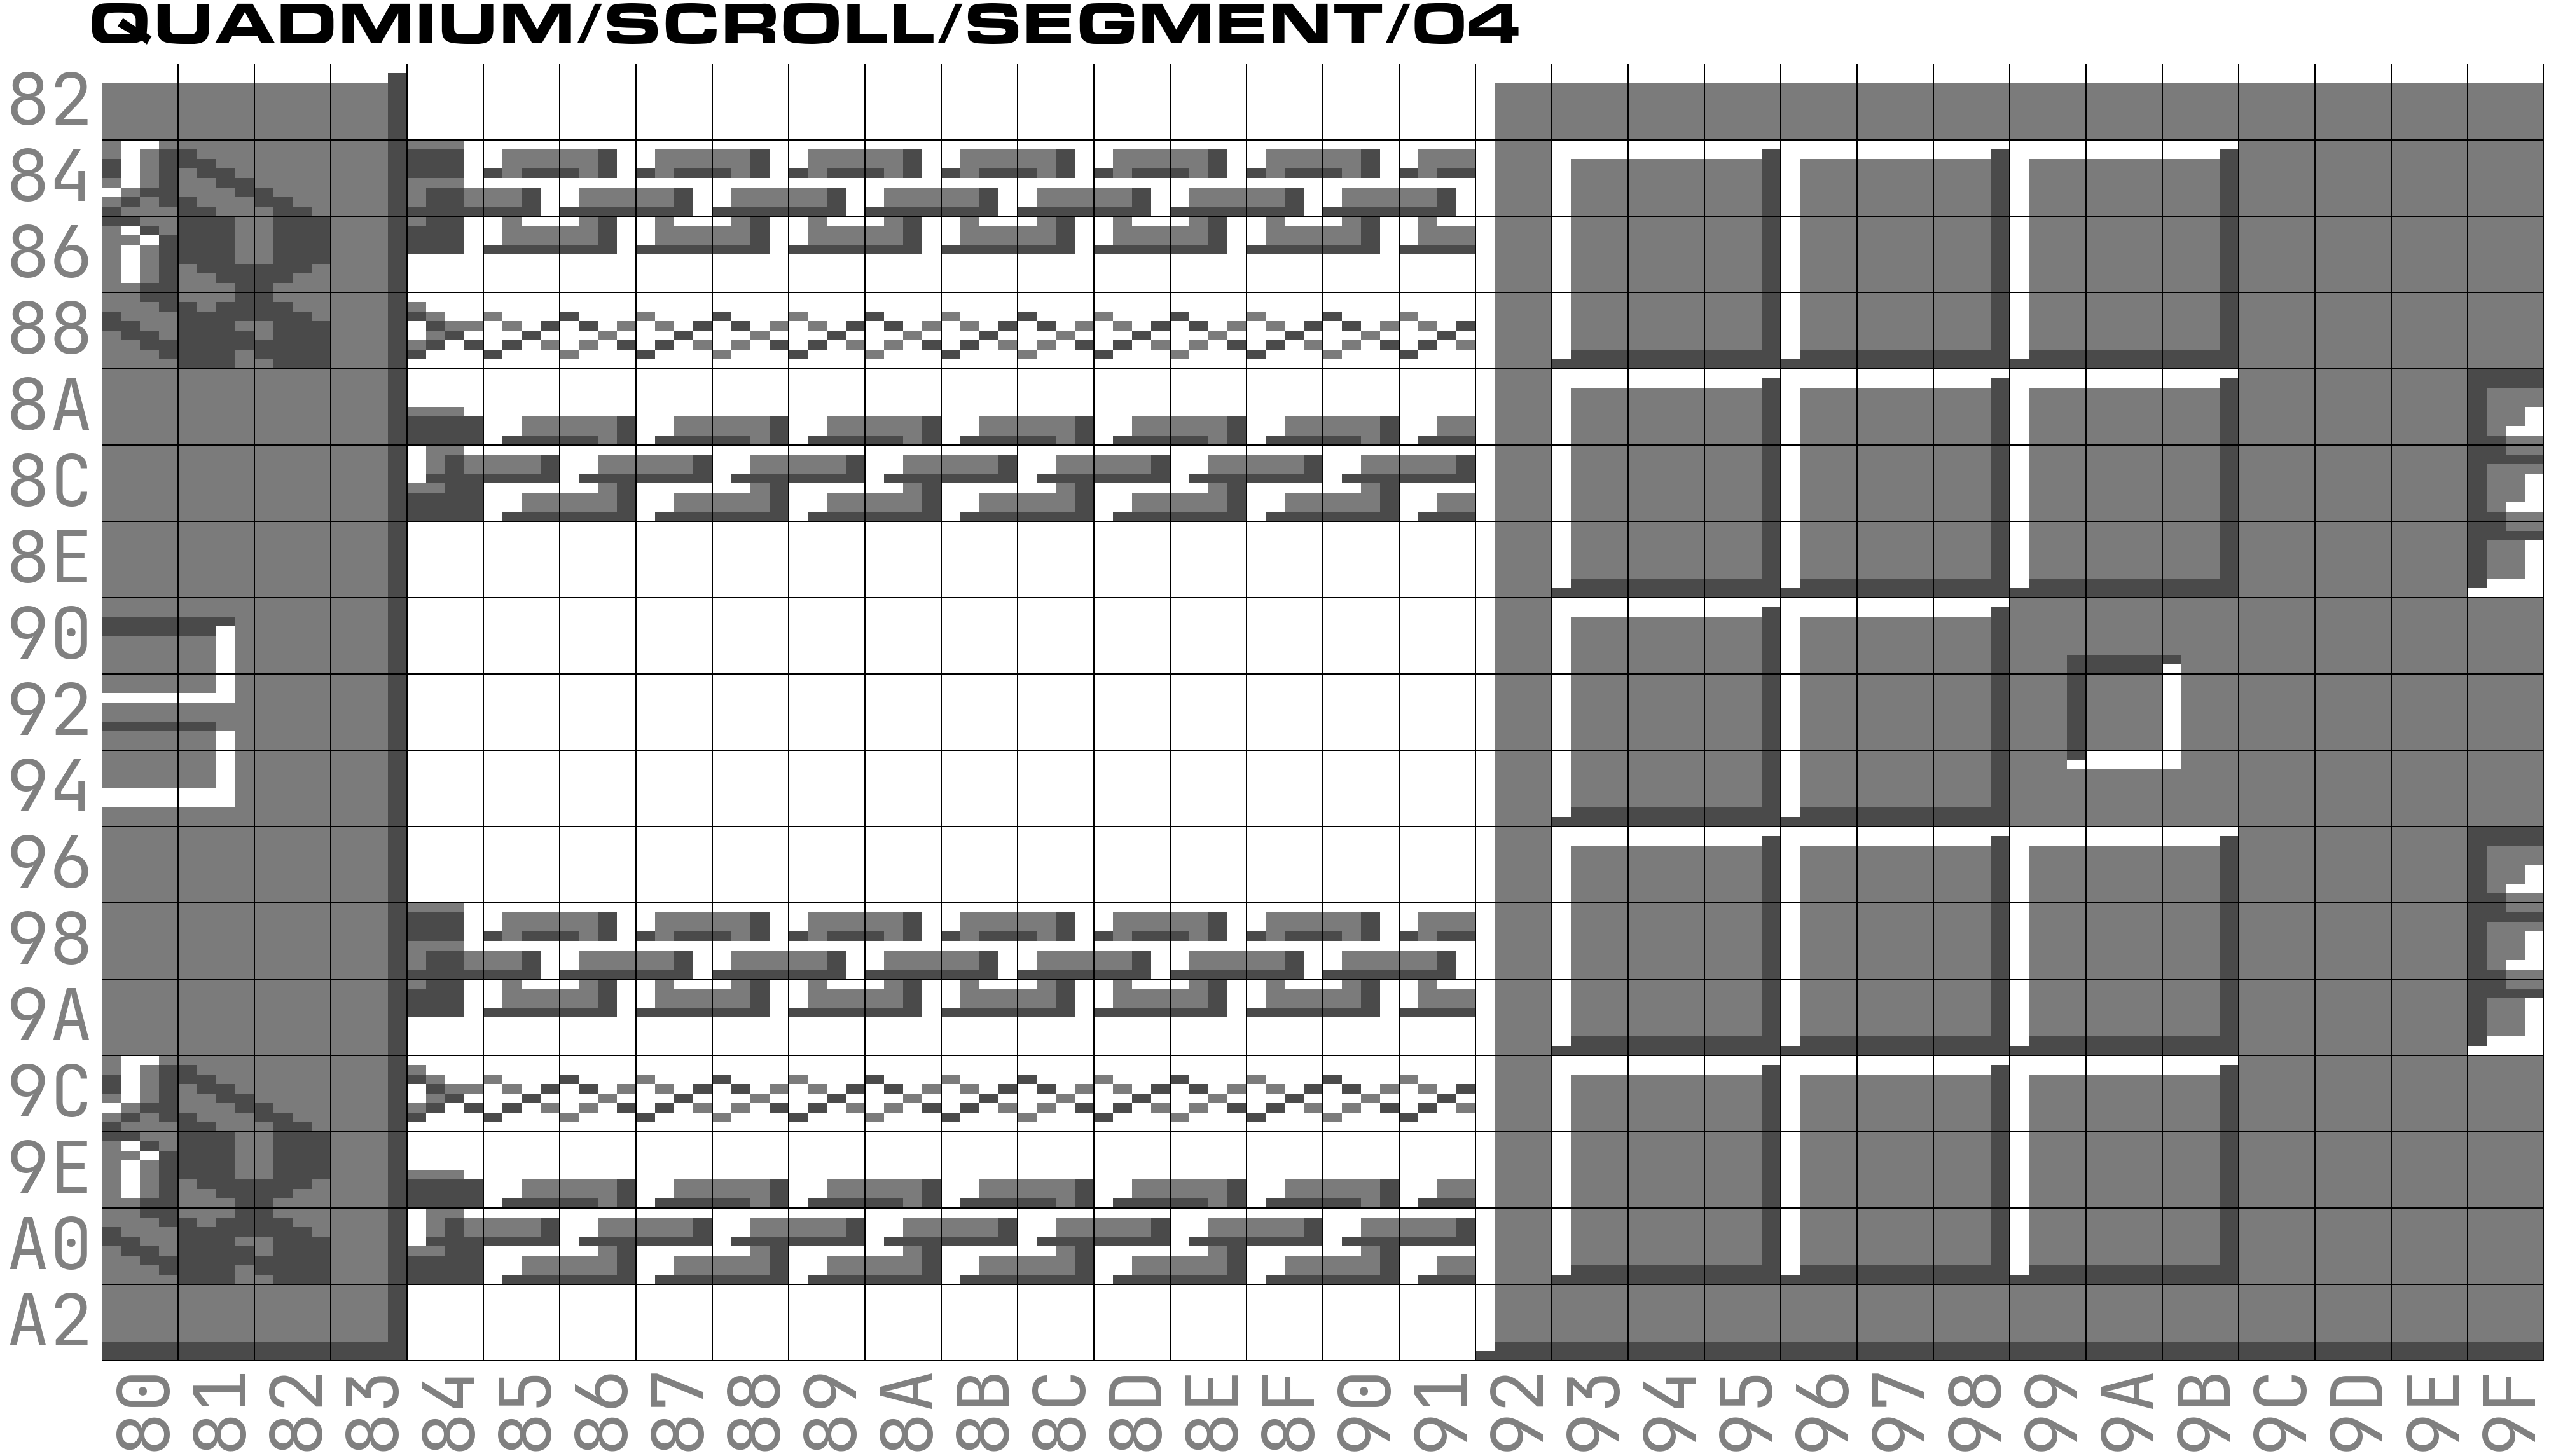
\includegraphics{src/scrolling/10_segment_4_0.png}%
    \end{adjustbox}
\end{figure}
\vspace{-0.4cm}

To arrive at a value of \icode{\$80} from a starting point of \icode{\$04}, what we need to do is multiply it by \icode{\$20}. 
Usually this would involve shifting a byte left 5 times, moving the bits up the byte. So for example a starting value of 4 (\icode{00000100}) would
move 5 positions to the left and give us a value of \icode{\$80} (\icode{10000000}). An alternative way would be to shift it right three (3) times
and let the bit wrap around to the front, so that \icode{00000100} wraps around to \icode{10000000}.

This latter approach is the one we take here, and the reason we do this is because our requirements come with an extra complication. 
We are not just figuring out an address for \icode{segment} by itself. We need to factor in \icode{pixelX} too, more specifically the
first 5 bits of \icode{pixelX}, which give us an offset between 0 and 32 within the segment.

The way we do this is by loading the last three bits of \icode{pixelX} with a value that will affect the bit shifting behaviour
of each of the three right shifts that we perform on both \icode{segment} and \icode{pixelX}. We store this updated version of
\icode{pixelX} in a new value \icode{scrollPositionLoPtr} and also shift it to the right three times. But we use a different method
for the shifting that takes in the side-effects of the \icode{pixelX} that manipulates its value. The key here is that the \icode{LSR}
(Logical Shift Right) operation we perform on the \icode{segment} value has a specific side-effect on the \icode{ROR} (Rotate Right) operations
we perform on \icode{scrollPositionLoPtr}: any time our \icode{LSR} operation pushes a \icode{0} off to the right any '1' bit rotated to the
right in \icode{scrollPositionLoPtr} is dropped. Any time our \icode{LSR} operation pushes a \icode{1} off to the right, the '1' bits rotated
off the right in \icode{scrollPositionLoPtr} are preserved and added back on to the front.

When we are done, it is \icode{scrollPositionLoPtr} that will have the value we desire: the memory address for the offset within the
segment that we need to scroll to. As you can see in the table below we give the full sequence of operations for example and end
up with the desired value of \icode{\$80}, having started from a segment value of \icode{\$04}:

\begin{figure}[H]
  {
    \setlength{\tabcolsep}{3.0pt}
    \setlength\cmidrulewidth{\heavyrulewidth} % Make cmidrule = 
    \begin{adjustbox}{width=11cm,center}
      \begin{tabular}{lcc}
        \toprule
        Instruction & Accumulator & \icode{scrollPositionLoPtr} \\
        \midrule
        \icode{LDA pixelX} & \icode{00000000} (00)  & \icode{00000000} (\icode{\$00}) \\
        \icode{CLC} & \icode{00000000} (00)  & \icode{00000000} (\icode{\$00}) \\
        \icode{ADC \#\$07}    & \icode{00000111}(07)  & \icode{00000000} (\icode{\$00}) \\
        \icode{STA scrollPositionLoPtr} & \icode{00000111}(07)  & \icode{00000111} (\icode{\$07}) \\
        \addlinespace
        \icode{LDA segment} & \icode{00000100} (04)  & \icode{00000111} (\icode{\$07}) \\
        \icode{ADC \#\$00}    & \icode{00000100} (04)  & \icode{00000111} (\icode{\$07}) \\
        \icode{LSR}         & \icode{00000010}  (02)  & \icode{00000111} (\icode{\$07}) \\
        \icode{ROR scrollPositionLoPtr}  &  \icode{00000010} (02) & \icode{00000011} (\icode{\$03}) \\
        \icode{LSR}         &  \icode{00000001} (01) & \icode{00000011} (\icode{\$03}) \\
        \icode{ROR scrollPositionLoPtr}  &  \icode{00000001} (01) & \icode{00000001} (\icode{\$01}) \\
        \icode{LSR}         &  \icode{00000000} (00) & \icode{00000001} (\icode{\$01}) \\
        \icode{ROR scrollPositionLoPtr}  &  \icode{00000000} (00) & \icode{10000000} (\icode{\$80}) \\
        \icode{AND \#\$01}    &  \icode{00000000} (00) & \icode{10000000} (\icode{\$80}) \\
        \icode{STA secondHalfOfMap} &  \icode{00000000} (00) & \icode{10000000} (\icode{\$80}) \\
        \addlinespace
        \bottomrule
      \end{tabular}
    \end{adjustbox}
  }
\end{figure}
\vspace{-0.4cm}

Returning to our earlier example where we had a \icode{segment} value of \icode{\$03} and a \icode{pixelX} value
of 214 (\icode{\$D6} in hex). We can follow the process again below. This time we can see that the '1' bits shifted off
to the right from our \icode{segment} value in the accumulator are allowing the '1' bits rotated off \icode{scrollPositionLoPtr}
to be preserved:

\begin{figure}[H]
  {
    \setlength{\tabcolsep}{3.0pt}
    \setlength\cmidrulewidth{\heavyrulewidth} % Make cmidrule = 
    \begin{adjustbox}{width=11cm,center}
      \begin{tabular}{lcc}
        \toprule
        Instruction & Accumulator & \icode{scrollPositionLoPtr} \\
        \midrule
        \icode{LDA pixelX} & \icode{\$D6}  & \icode{00000000} (000, \icode{\$00}) \\
        \icode{CLC} & \icode{\$D6}  & \icode{00000000} (000, \icode{\$00}) \\
        \icode{ADC \#\$07}    & \icode{\$DD}  & \icode{00000000} (000, \icode{\$00}) \\
        \icode{STA scrollPositionLoPtr} & \icode{\$DD}  & \icode{11011101} (221, \icode{\$DD}) \\
        \addlinespace
        \icode{LDA segment} & \icode{\$03}  & \icode{11011101} (221, \icode{\$DD}) \\
        \icode{ADC \#\$00}    & \icode{\$03}  & \icode{11011101} (221, \icode{\$DD}) \\
        \icode{LSR}         & \icode{\$01}   & \icode{11011101} (221, \icode{\$DD}) \\
        \icode{ROR scrollPositionLoPtr}  &  \icode{\$01} & \icode{11101110} (238, \icode{\$EE}) \\
        \icode{LSR}         &  \icode{\$00} & \icode{11101110} (238, \icode{\$EE}) \\
        \icode{ROR scrollPositionLoPtr}  &  \icode{\$00} & \icode{11110111} (247, \icode{\$F7}) \\
        \icode{LSR}         &  \icode{\$00} & \icode{11110111} (247, \icode{\$F7}) \\
        \icode{ROR scrollPositionLoPtr}  &  \icode{\$00} & \icode{01111011} (123, \icode{\$7B}) \\
        \icode{AND \#\$01}    &  \icode{\$00} & \icode{01111011} (123, \icode{\$7B}) \\
        \icode{STA secondHalfOfMap} &  \icode{\$00} & \icode{01111011} (123, \icode{\$7B}) \\
        \addlinespace
        \bottomrule
      \end{tabular}
    \end{adjustbox}
  }
\end{figure}
\vspace{-0.4cm}

Our end result is \icode{\$7B}, which  gives us a memory address of \icode{\$827B}. This is the desired position,
26 characters to the right of the segment boundary at \icode{\$8260}:
\begin{figure}[H]
    \begin{adjustbox}{width=13.3cm,left}
      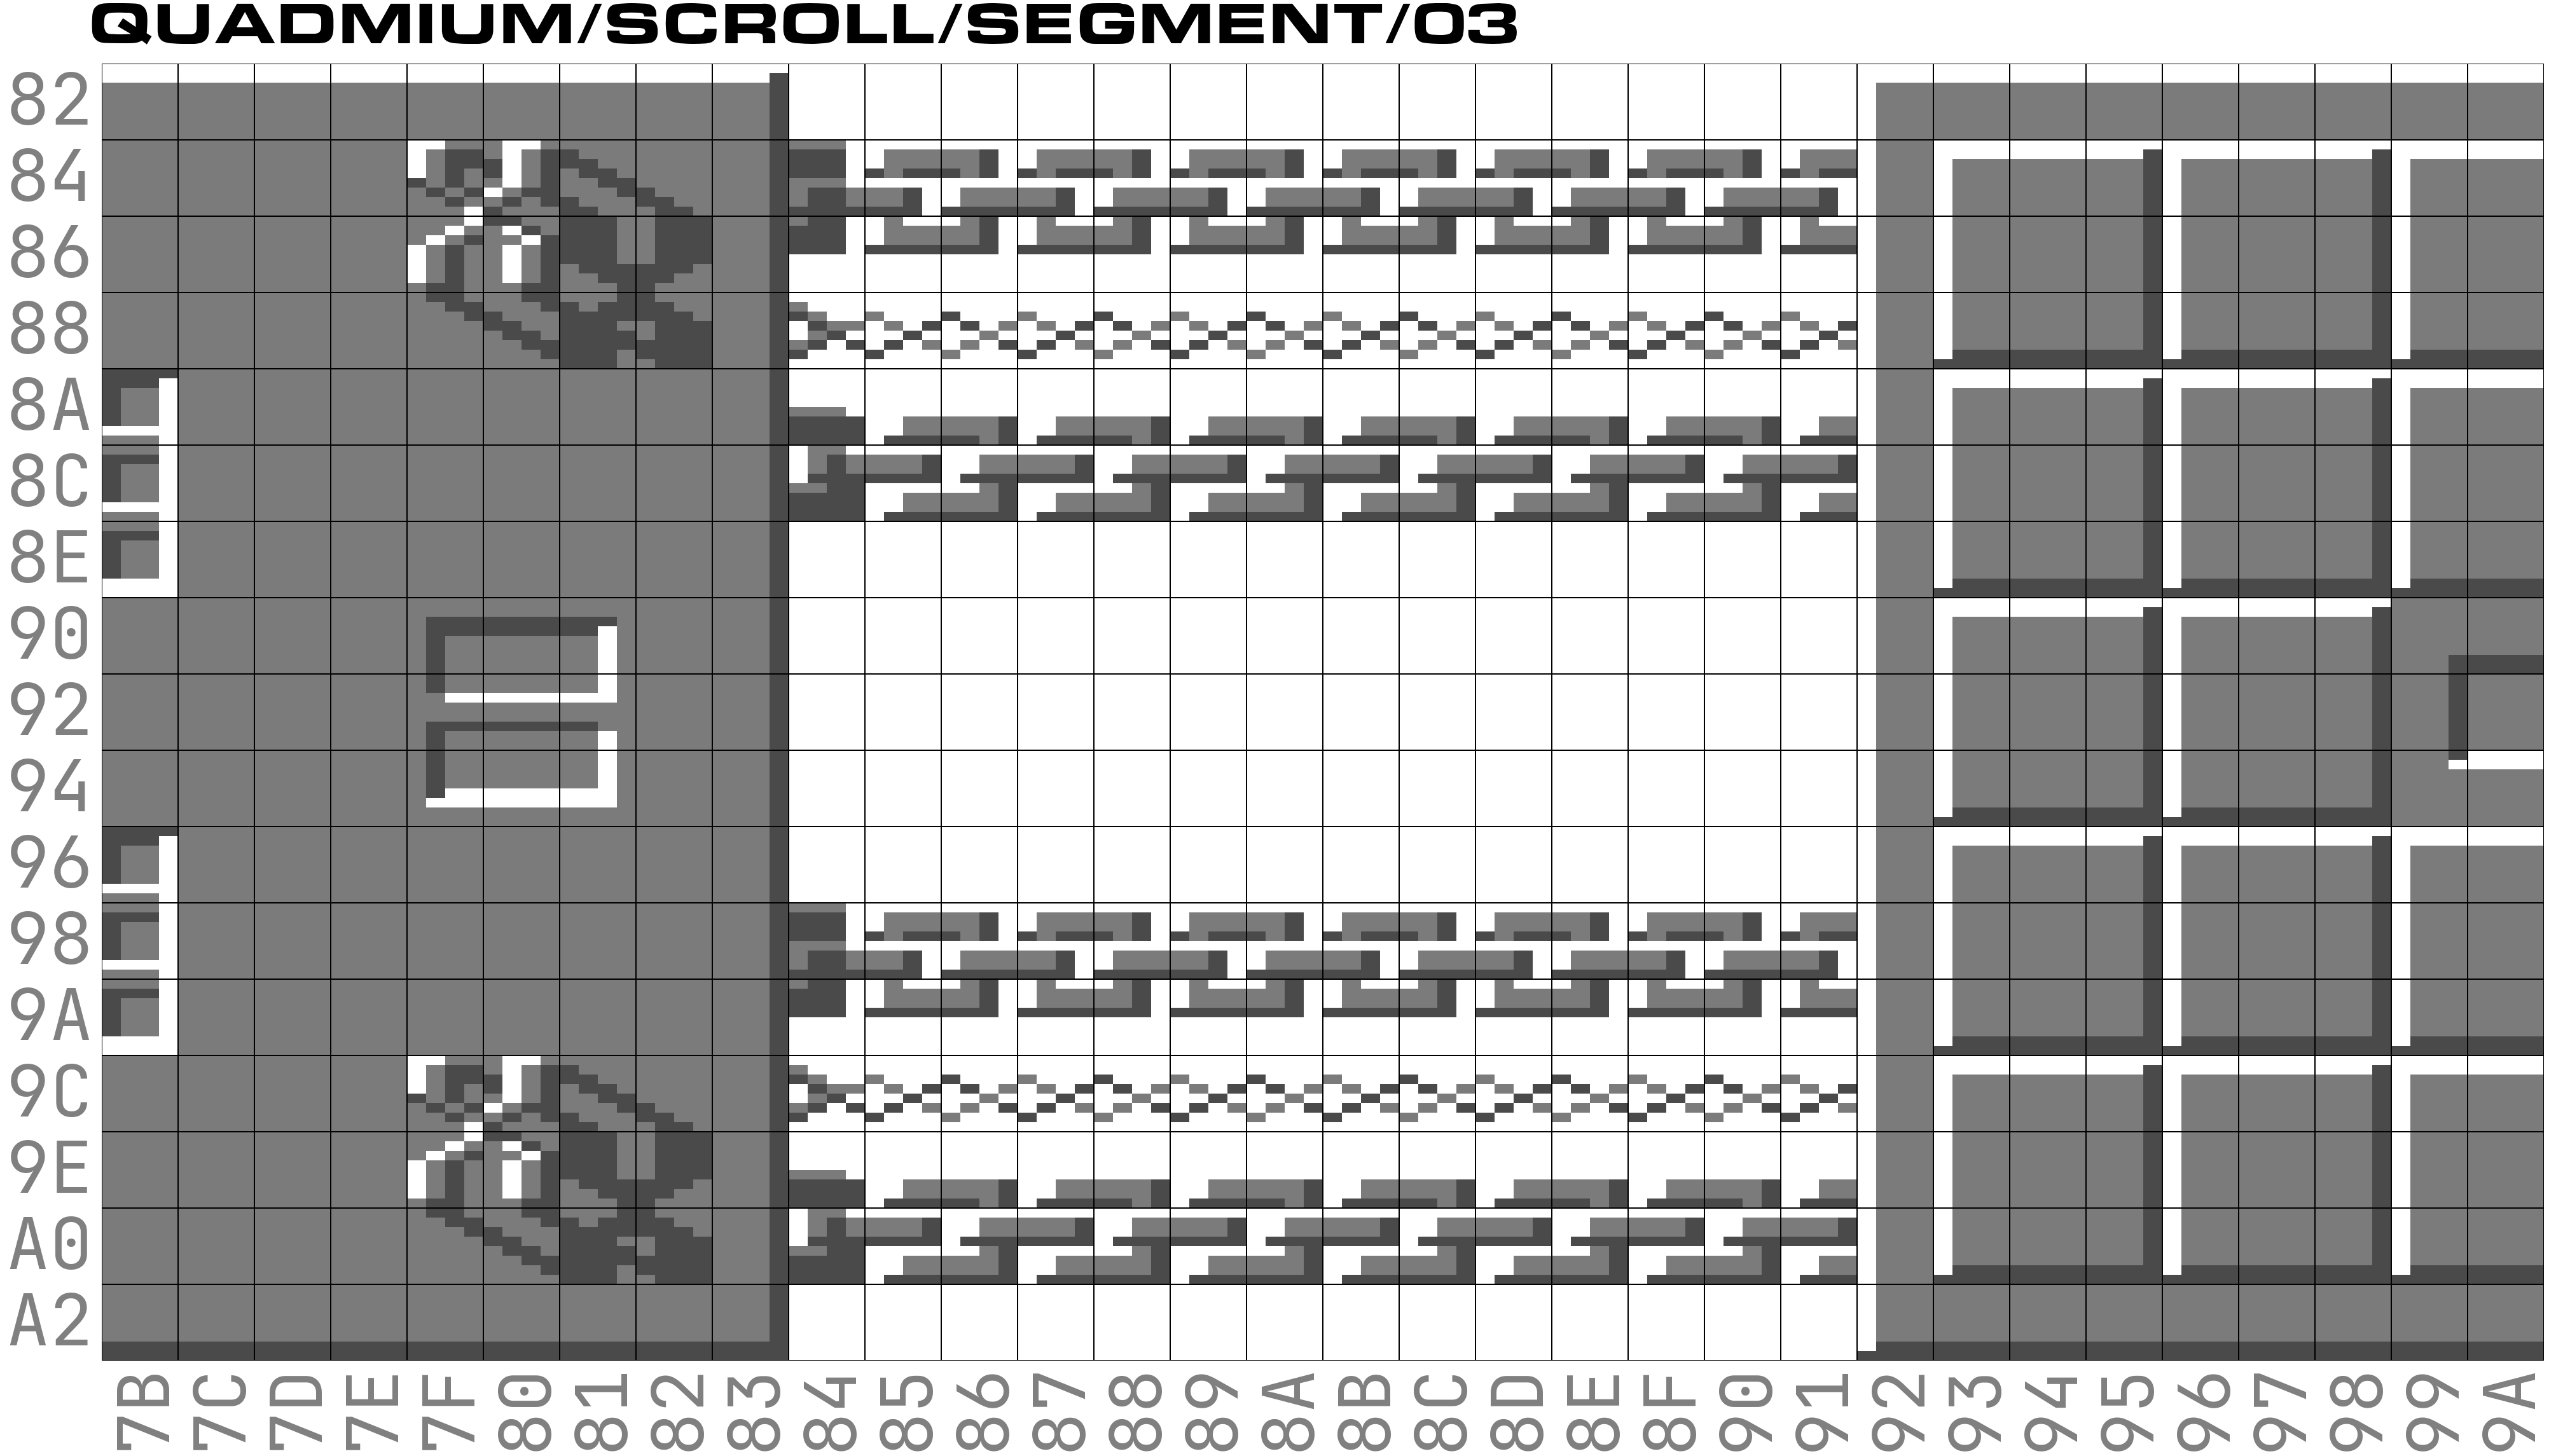
\includegraphics{src/scrolling/10_segment_3_27.png}%
    \end{adjustbox}
\end{figure}
\vspace{-0.4cm}
We've reproduced the routine that the table above refers to opposite. This is the first half
of the \icode{ScrollShipSurface} and it has achieved its most important function: figuring
out the address of the section of the playfield to display.


\clearpage
\begin{lstlisting}
;---------------------------------------------------------------------
; This routine figures out the part of the playfield to display on the
; screen using 'segment' and 'pixelX'. It's end result is an address in
; screenDataLoPtr/screenDataHiPtr that points to the top left of
; the section of the playfield to display. The second half of the
; routine is on the following page.
;---------------------------------------------------------------------
ScrollShipSurface
  ; Store pixelX in scrollPositionLoPtr. We add 7 so that we ensure
  ; there are three bits at the end. These will get shifted out below
  ; but are necessary to ensure we merge pixelX with the segment value
  ; correctly.
  LDA pixelX              ; Load pixelX to A.
  CLC                     ; Clear the carry bit.
  ADC #$07                ; Add three bits '111'.
  STA scrollPositionLoPtr ; Store result in scrollPositionLoPtr.

  ; Figure out the memory address that we want to snap to and display.
  ; The routine below effectively performs the following mapping
  ; for each value of segment and adds the first 5 bits of pixelX
  ; as an offset on top:
  ;
  ; $X0 -> 8200, $X1 -> 8220, $X2 -> 8240, $X3 -> 8260
  ; $X4 -> 8280, $X5 -> 82A0, $X6 -> 82C0, $X7 -> 82F0
  ; $X8 -> 8300, $X9 -> 8320, $XA -> 8340, $XB -> 8360
  ; $XC -> 8380, $XD -> 83A0, $XE -> 83C0, $XF -> 83F0
  ;
  LDA segment             ; Load the segment value to A.
  ADC #$00                ; Add the carry bit.
  LSR                     ; Shift 'segment' 1 bit to the right.
  ROR scrollPositionLoPtr ; Rotate scrollPositionLoPtr 1 bit to the right.
  LSR                     ; Shift 'segment' 1 bit to the right.
  ROR scrollPositionLoPtr ; Rotate scrollPositionLoPtr 1 bit to the right.
  LSR                     ; Shift 'segment' 1 bit to the right.
  ROR scrollPositionLoPtr ; Rotate scrollPositionLoPtr 1 bit to the right.

  ; Use the last bit of the Accumulator to tell us whether we're in the
  ; first half of the map ($8200) or the second half ($8300).
  AND #$01                ; Get the last bit.
  STA secondHalfOfMap     ; Store it in secondHalfOfMap.

  ; Now that we have figured out the address in the playfield that we
  ; want to display, we can store it in the variables we will use
  ; for actually writing that part of the playfield to the screen.
  ; screenDataLoPtr/screenDataHiPtr will be the 'source' address
  ; that we start from when writing the 17 rows of playfield that are 38
  ; bytes wide.
  LDA #$82                ; Get the start of the playfield memory address.
  ORA secondHalfOfMap     ; Add 1 for the second half if necessary.
  STA screenDataHiPtr     ; Store as the 1st part of source address.
  LDA scrollPositionLoPtr ; Load final value of scrollPositionLoPtr
  STA screenDataLoPtr     ; Store as the 2nd part of source address.
\end{lstlisting}
\vspace*{\fill}
\clearpage

The second half of the routine has a much more straightforward task: writing the selected
frame to the screen. Although we split the game's map into sixteen segments of 32 bytes in
width, this was a convenience for our divide and conquer approach to determining where on
the map to select our frame for display. The frame that we actually display is wider than
32 bytes, clocking in at 40 bytes wide in total.

Glancing through the routine opposite it should be possible for you to see that we draw
the screen in step-wise fashion starting at the top left, and working across and down. So
in our example where we have selected a memory address of \icode{\$827B} as the top left position
of the playfield to start our drawing from, we begin by drawing the first character in 
\icode{DrawNextCharacter}:
\begin{figure}[H]
    \begin{adjustbox}{width=13.3cm,left}
      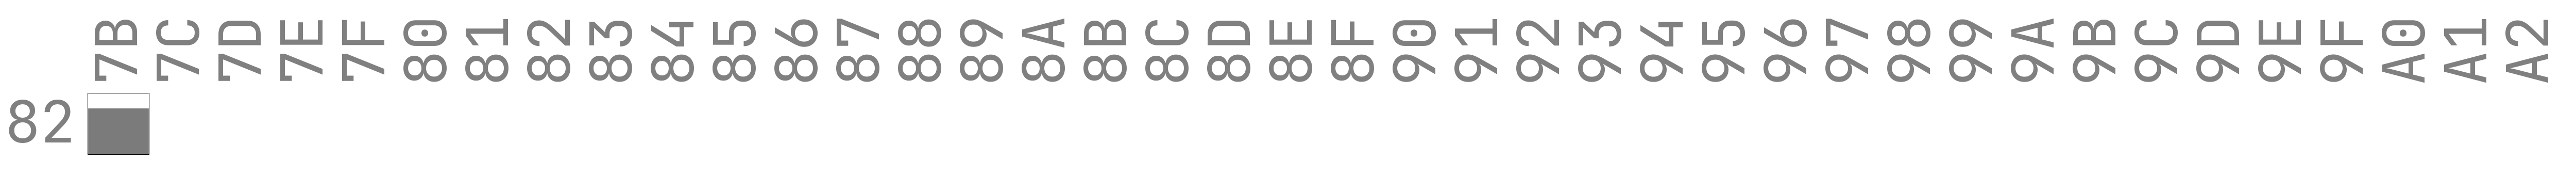
\includegraphics{src/scrolling/drawing/10_diagram_3_1_1_diagram.png}%
    \end{adjustbox}
\end{figure}
\vspace{-0.8cm}
We then continue looping in \icode{DrawNextCharacter} drawing another character:

\begin{figure}[H]
    \begin{adjustbox}{width=13.3cm,left}
      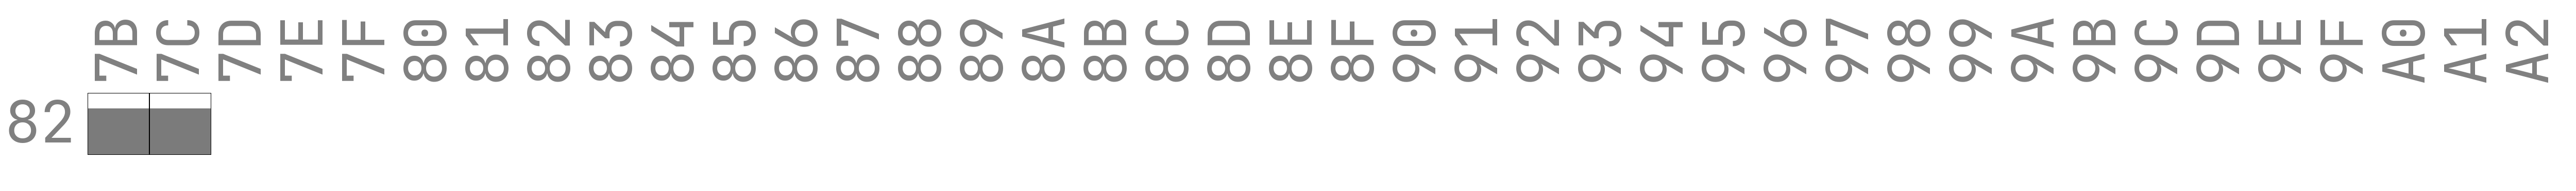
\includegraphics{src/scrolling/drawing/10_diagram_3_1_2_diagram.png}%
    \end{adjustbox}
\end{figure}
\vspace{-0.8cm}
Followed by another:

\begin{figure}[H]
    \begin{adjustbox}{width=13.3cm,left}
      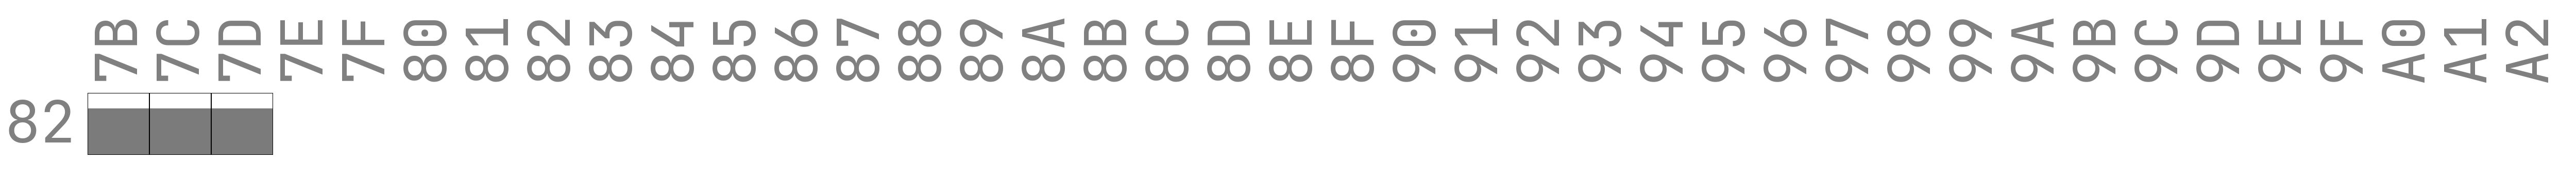
\includegraphics{src/scrolling/drawing/10_diagram_3_1_3_diagram.png}%
    \end{adjustbox}
\end{figure}
\vspace{-0.8cm}

Until the whole line is filled:
\begin{figure}[H]
    \begin{adjustbox}{width=13.3cm,left}
      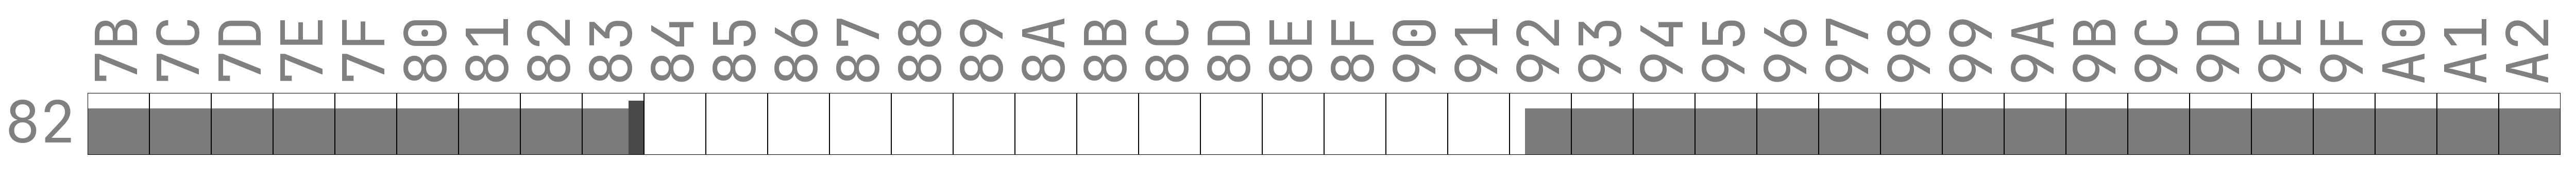
\includegraphics{src/scrolling/drawing/10_diagram_3_1_40_diagram.png}%
    \end{adjustbox}
\end{figure}
\vspace{-0.8cm}

We then move to the next line by jumping back to \icode{DrawRows} and drawing
another line below it. Notice that as our playfield is 512 bytes wide, the
start address of the line has incremented from \icode{\$827B} to \icode{\$847B}:

\begin{figure}[H]
    \begin{adjustbox}{width=13.3cm,left}
      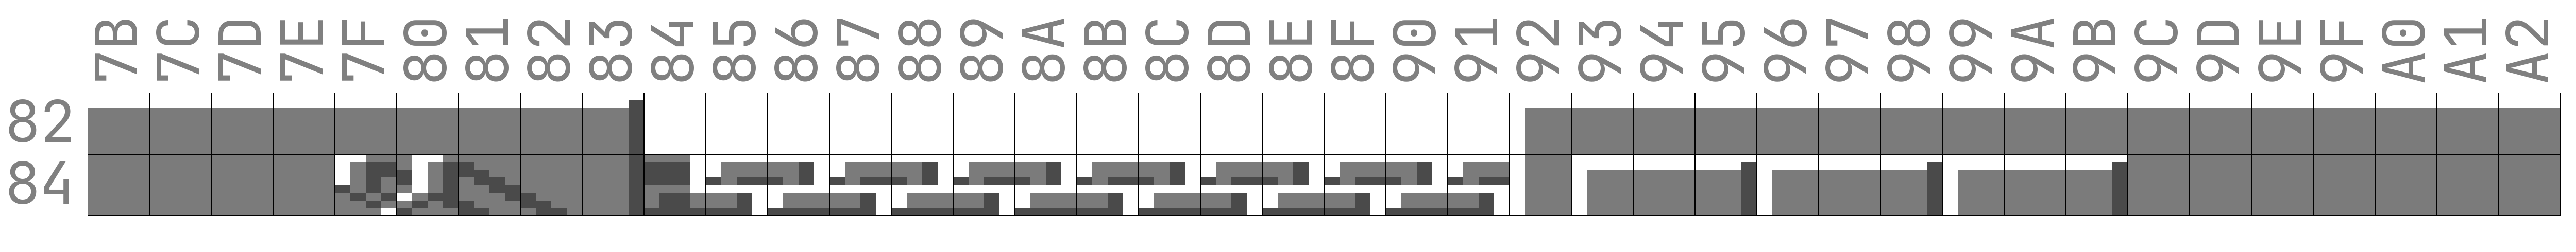
\includegraphics{src/scrolling/drawing/10_diagram_3_2_40_diagram.png}%
    \end{adjustbox}
\end{figure}
\vspace{-0.8cm}

We then repeat this process, adding more and more lines, one at a time:
\begin{figure}[H]
    \begin{adjustbox}{width=13.3cm,left}
      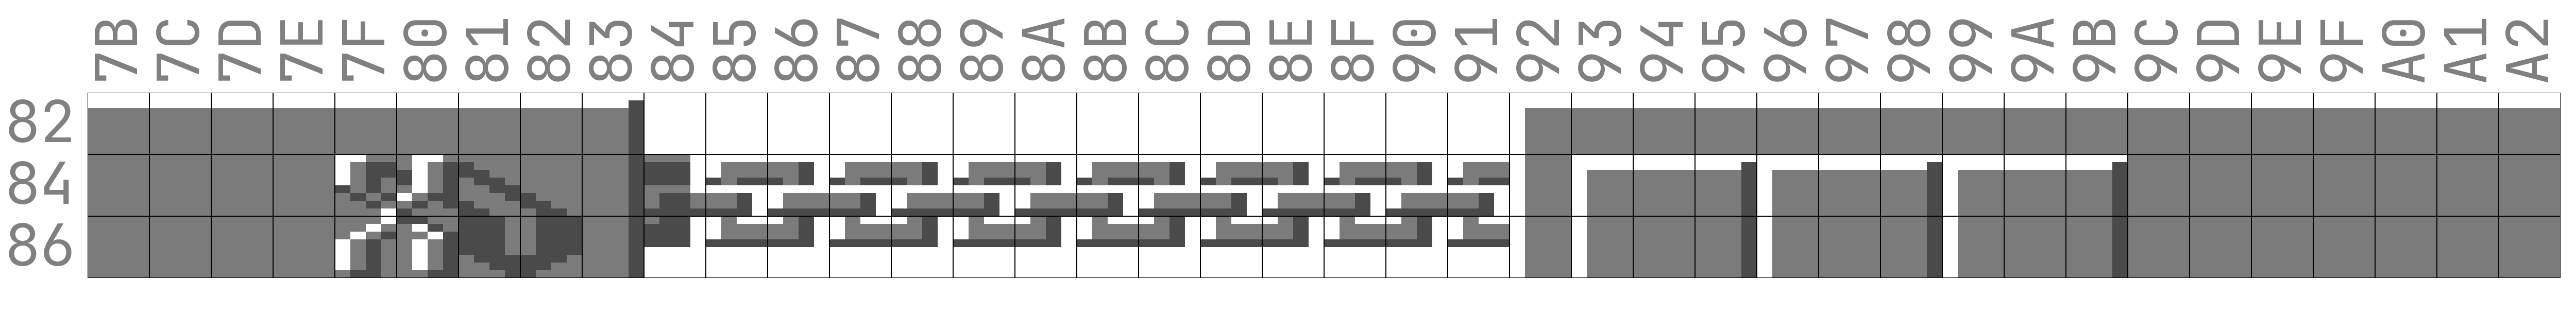
\includegraphics{src/scrolling/drawing/10_diagram_3_3_40_diagram.png}%
    \end{adjustbox}
\end{figure}
\vspace{-0.8cm}

\clearpage
\begin{lstlisting}
;---------------------------------------------------------------------
; This second half of the ScrollShipSurface routine looks after drawing
; to the screen the segment we selected in the first half. Note that the
; use of pointers to positions within the code (e.g. screenDataLoPtr/
; screenDataHiPtr) makes this code 'self-mutating'.
;---------------------------------------------------------------------
ScrollShipSurfaceContinued
  ; Get the high and low byte of the RAM used to display the screen
  ; and store it in screenRAMLoPtr/screenRAMHiPtr.
  LDA #>screenRAM           ; Load high byte of the screen RAM.
  STA screenRAMHiPtr        ; Store in screenRAMHiPtr
  LDA #<screenRAM           ; Load low byte of the screen RAM.
  STA screenRAMLoPtr        ; Store in screenRAMLoPtr

  ; This loops through all 40 columns of all 17 rows of the screen
  ; and draws the selected frame of the surface on it. The inner loop
  ; is DrawNextCharacter. The outer loop is DrawRow. Note how we update
  ; the address referenced by screenData and screenRAM directly in the code
  ; itself using the screenDataLoPtr/screenDataHiPtr and screenRAMLoPtr/
  ; screenRAMHiPtr references.
  LDX #17                   ; Draw 17 rows.
DrawRow   
  LDY #40                   ; Draw 40 characters in each row.
DrawNextCharacter   
  ; screenDataLoPtr/screenDataHiPtr are pointers to screenData, allowing
  ; us to mutate the address screenData points to.
  screenDataLoPtr =*+$01    ; Pointer to low byte.
  screenDataHiPtr =*+$02    ; Pointer to high byte.
  LDA screenData,Y          ; Load the character in screen data.

  ; screenRAMLoPtr/screenRAMHiPtr are pointers to screenRAM, 
  ; allowing us to mutate the address screenRAM points to.
  screenRAMLoPtr  =*+$01    ; Pointer to low byte.
  screenRAMHiPtr  =*+$02    ; Pointer to high byte.
  STA screenRAM,Y           ; Write the character to screen.
  DEY                       ; Go to next character in row.
  BPL DrawNextCharacter     ; Loop until last character in row.

  DEX                       ; Go to next row.
  BEQ Finished              ; If reached last row, we're done.
  INC screenDataHiPtr       ; Move to next row of screen data, e.g. from
  INC screenDataHiPtr       ; position $8220 to position $8420.

  LDA screenRAMLoPtr        ; Load the screenRAMLoPtr
  CLC                       ; Clear the carry bit.
  ADC #40                   ; Add 40 to go to next row on screen. 
  STA screenRAMLoPtr        ; Update screenRAMLoPtr with next row.
  BCC DrawRow               ; Do the next row.
  INC screenRAMHiPtr        ; Move the next high byte in screen RAM.
  JMP DrawRow               ; Do the next row.

Finished
  RTS                       ; We're finished, return from ScrollShipSurface.
\end{lstlisting}
\clearpage

Building up a stack of lines one by one:
\begin{figure}[H]
    \begin{adjustbox}{width=13.3cm,left}
      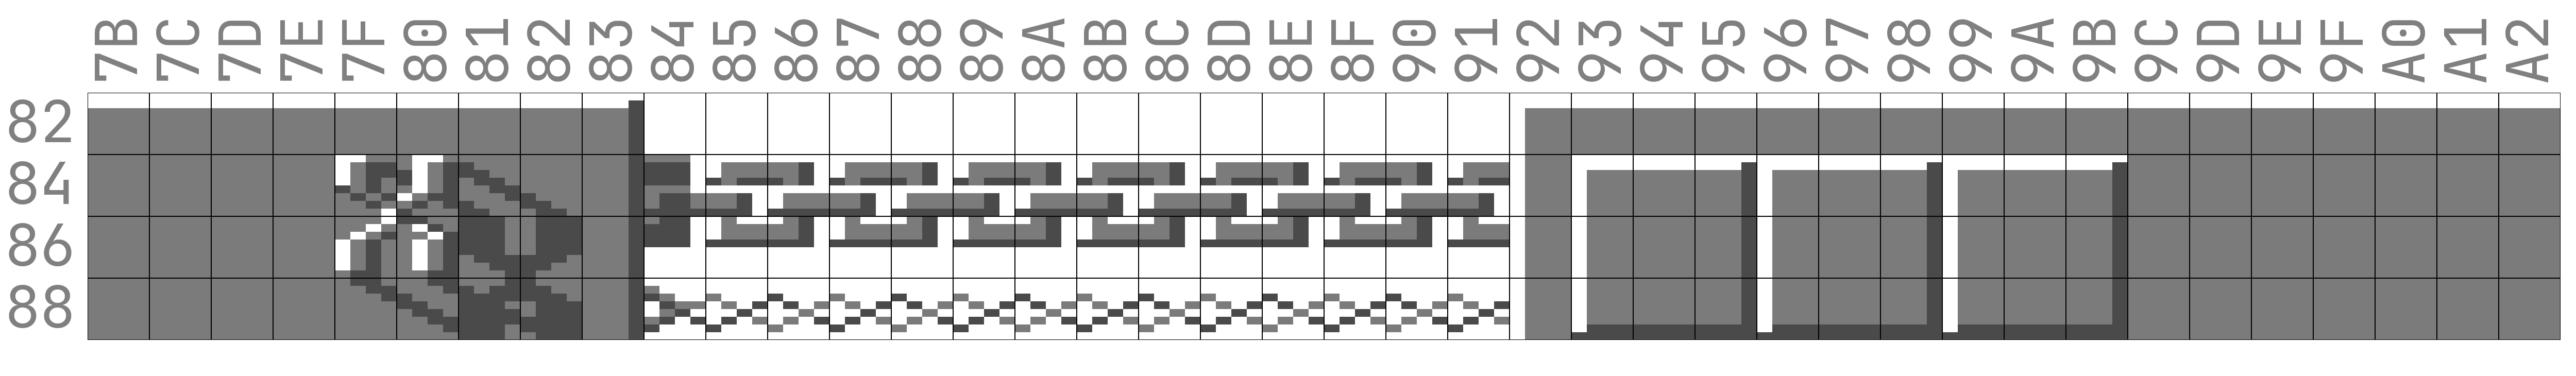
\includegraphics{src/scrolling/drawing/10_diagram_3_4_40_diagram.png}%
    \end{adjustbox}
\end{figure}
\vspace{-0.4cm}
\begin{figure}[H]
    \begin{adjustbox}{width=13.3cm,left}
      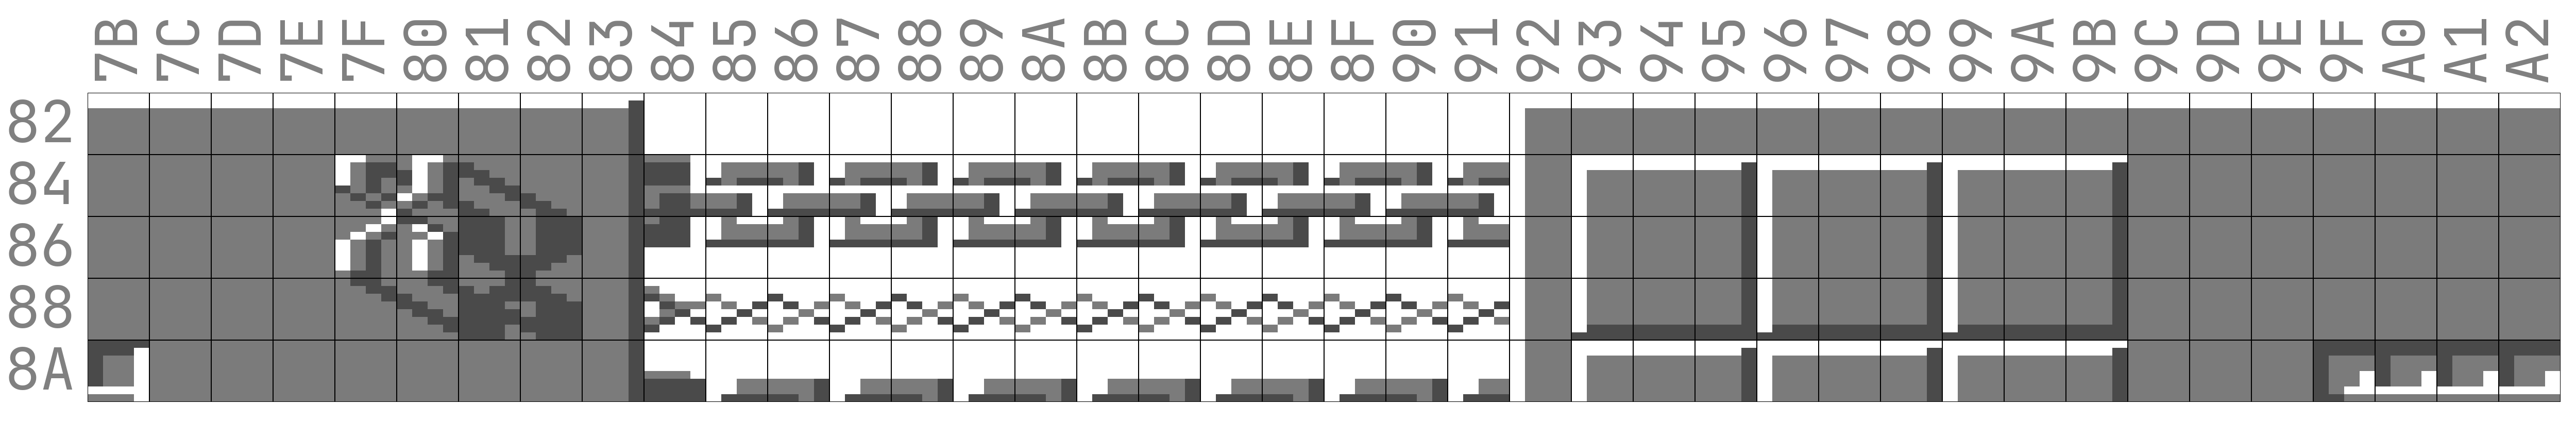
\includegraphics{src/scrolling/drawing/10_diagram_3_5_40_diagram.png}%
    \end{adjustbox}
\end{figure}
\vspace{-0.4cm}
\begin{figure}[H]
    \begin{adjustbox}{width=13.3cm,left}
      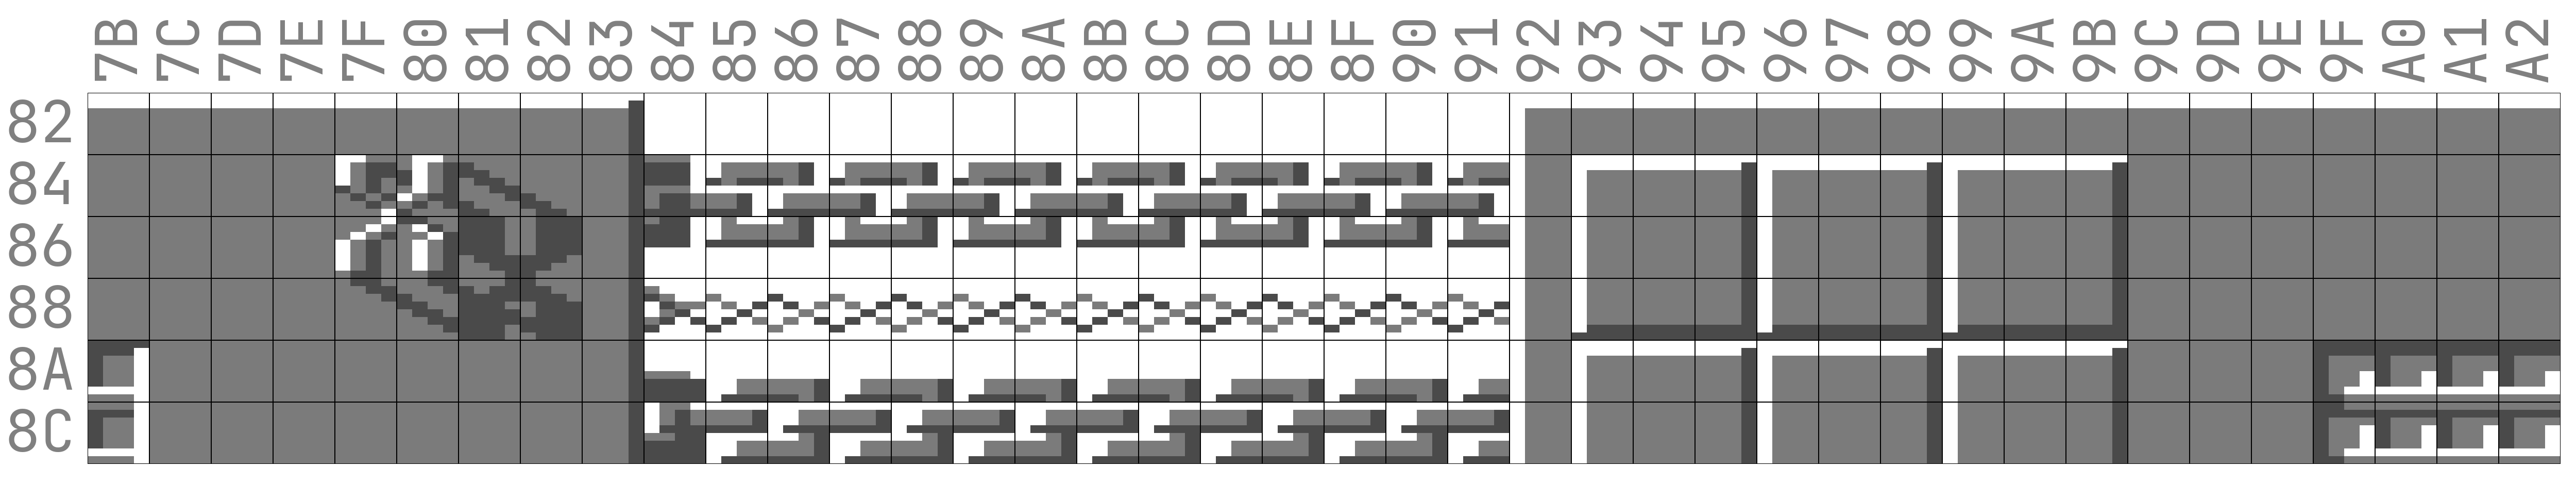
\includegraphics{src/scrolling/drawing/10_diagram_3_6_40_diagram.png}%
    \end{adjustbox}
\end{figure}
\vspace{-0.4cm}
Until finally we have a full screen:
\begin{figure}[H]
    \begin{adjustbox}{width=13.3cm,left}
      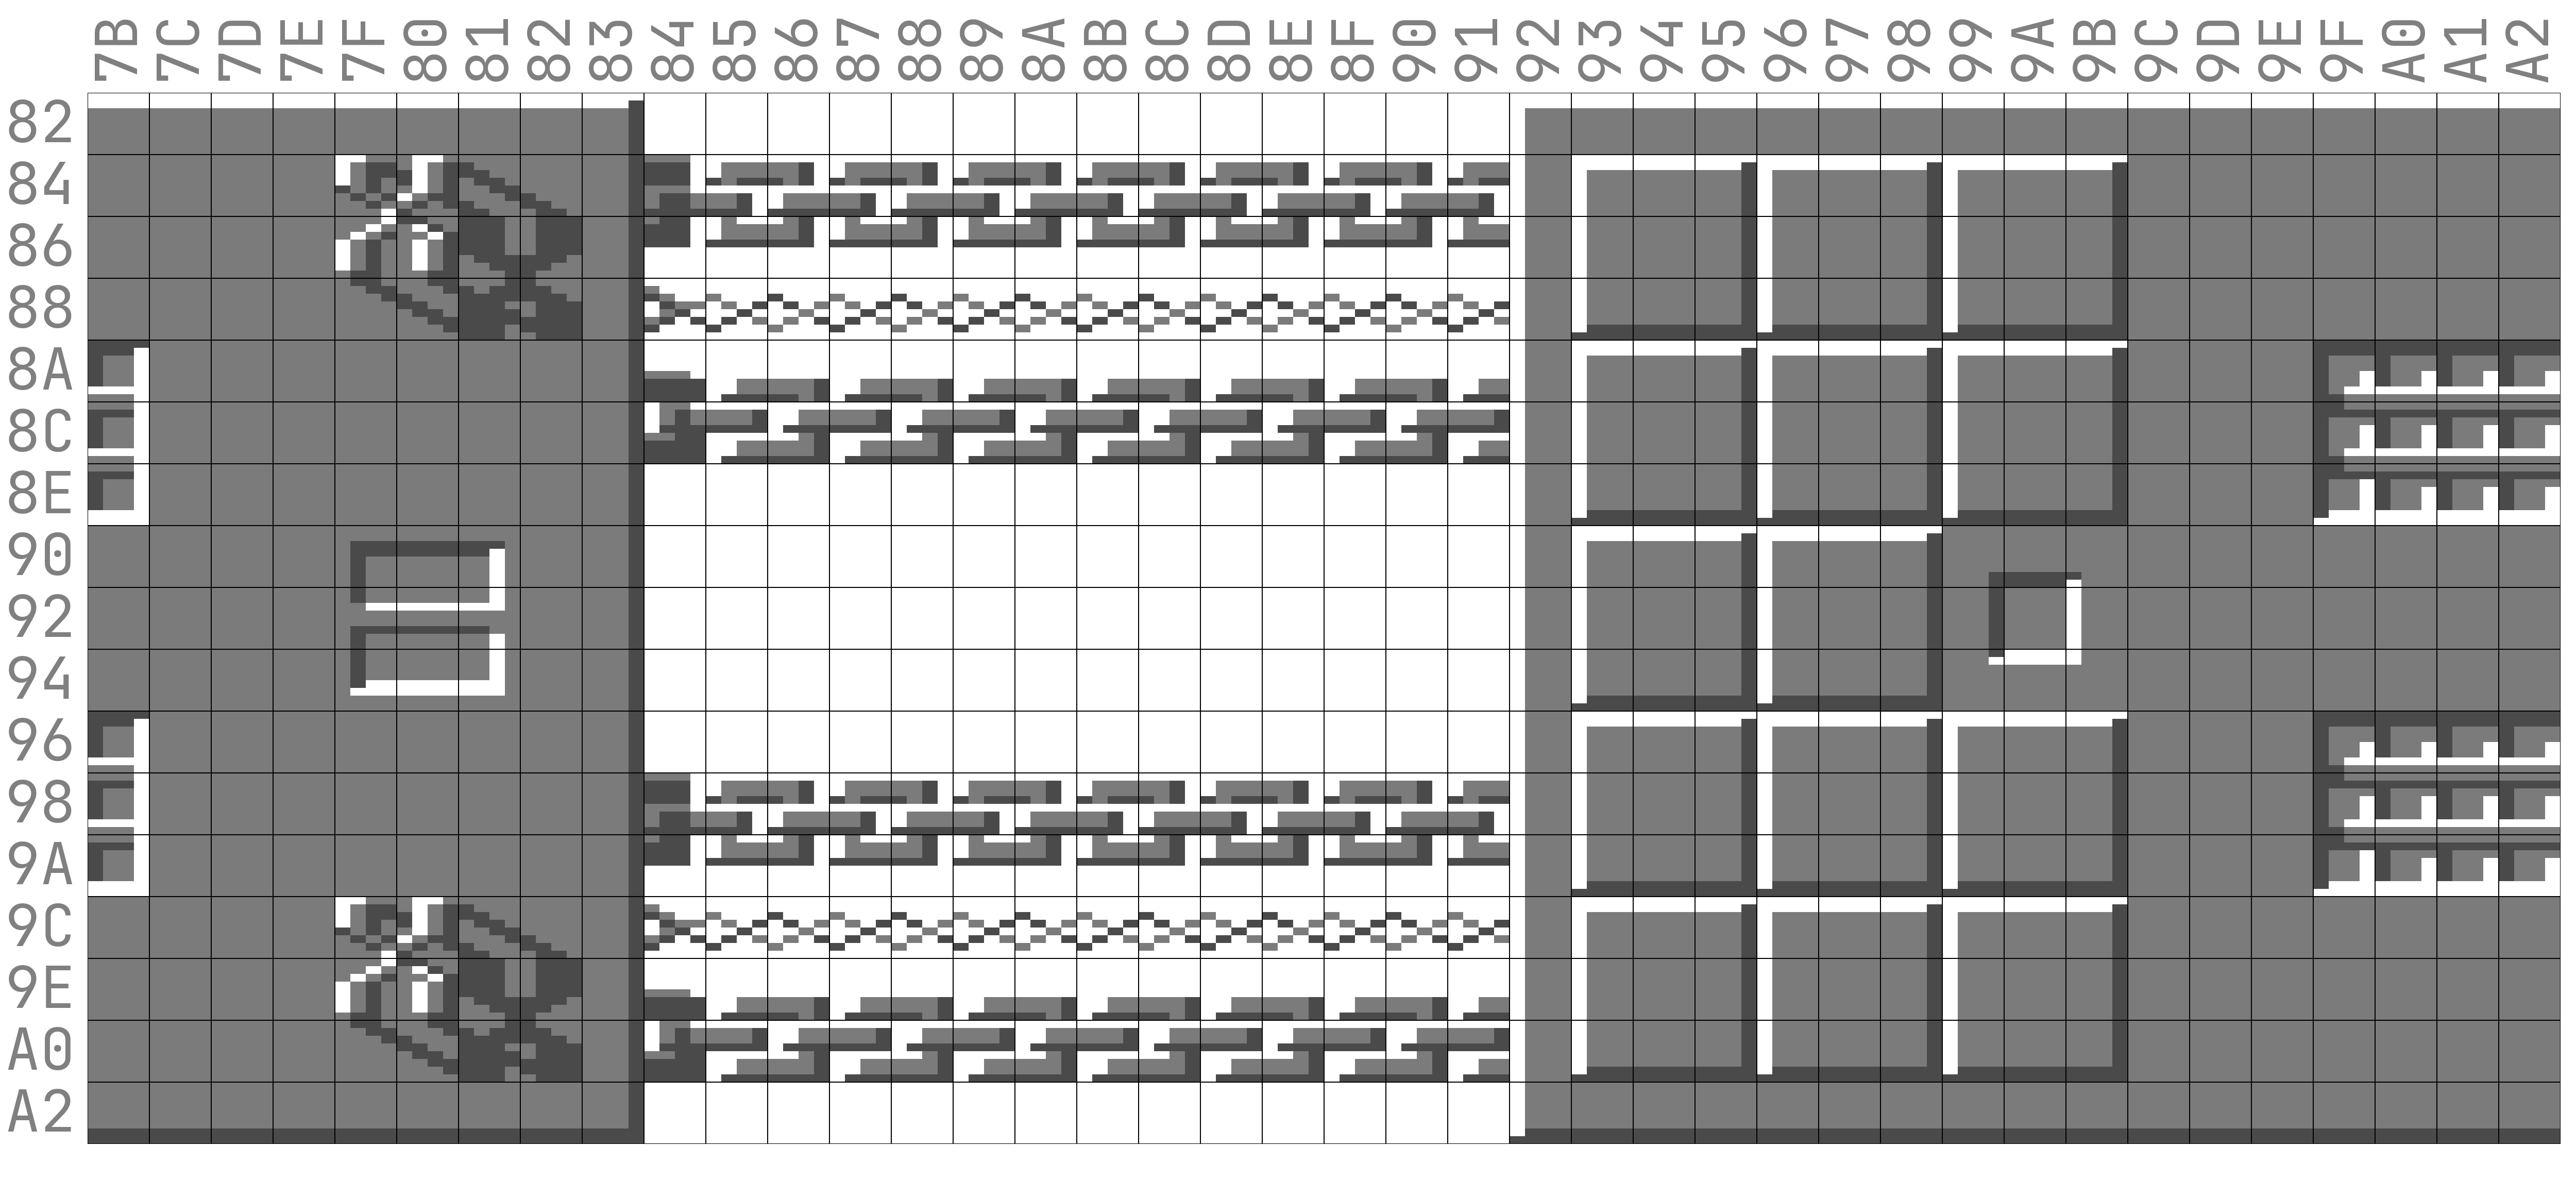
\includegraphics{src/scrolling/drawing/10_diagram_3_17_40_diagram.png}%
    \end{adjustbox}
\end{figure}
\vspace{-0.4cm}

And with that we have successully achieved a frame of 'scroll' by feeding our
routine an arbitrary \icode{segment} and \icode{pixelX} value. The entire process
is so compact and efficient that calling this many times per second is possible,
and so enables the silky smooth (and rapid) scrolling that is the hallmark of
\textit{Uridium}.


%\begin{figure}[H]
%  {
%    \setlength{\tabcolsep}{3.0pt}
%    \setlength\cmidrulewidth{\heavyrulewidth} % Make cmidrule = 
%    \begin{adjustbox}{width=11cm,center}
%      \begin{tabular}{lcc}
%        \toprule
%        Instruction & Accumulator & \icode{scrollPositionLoPtr} \\
%        \midrule
%        \icode{LDA pixelX} & \icode{\$00}  & \icode{00000000} (000, \icode{\$00}) \\
%        \icode{CLC} & \icode{\$00}  & \icode{00000000} (000, \icode{\$00}) \\
%        \icode{ADC \#\$07}    & \icode{\$07}  & \icode{00000000} (000, \icode{\$00}) \\
%        \icode{STA scrollPositionLoPtr} & \icode{\$07}  & \icode{00000111} (007, \icode{\$07}) \\
%        \addlinespace
%        \icode{LDA segment} & \icode{\$03}  & \icode{00000111} (007, \icode{\$07}) \\
%        \icode{ADC \#\$00}    & \icode{\$03}  & \icode{00000111} (007, \icode{\$07}) \\
%        \icode{LSR}         & \icode{\$01}   & \icode{00000111} (007, \icode{\$07}) \\
%        \icode{ROR scrollPositionLoPtr}  &  \icode{\$01} & \icode{10000011} (131, \icode{\$83}) \\
%        \icode{LSR}         &  \icode{\$00} & \icode{10000011} (131, \icode{\$83}) \\
%        \icode{ROR scrollPositionLoPtr}  &  \icode{\$00} & \icode{11000001} (193, \icode{\$C1}) \\
%        \icode{LSR}         &  \icode{\$00} & \icode{11000001} (193, \icode{\$C1}) \\
%        \icode{ROR scrollPositionLoPtr}  &  \icode{\$00} & \icode{01100000} (096, \icode{\$60}) \\
%        \icode{AND \#\$01}    &  \icode{\$00} & \icode{01100000} (096, \icode{\$60}) \\
%        \icode{STA secondHalfOfMap} &  \icode{\$00} & \icode{01100000} (096, \icode{\$60}) \\
%        \addlinespace
%        \bottomrule
%      \end{tabular}
%    \end{adjustbox}
%  }
%\end{figure}
%\begin{figure}[H]
%  {
%    \setlength{\tabcolsep}{3.0pt}
%    \setlength\cmidrulewidth{\heavyrulewidth} % Make cmidrule = 
%    \begin{adjustbox}{width=13cm,center}
%      \begin{tabular}{ccccccccc}
%        \toprule
%        Segment & Address & Segment & Address & Segment & Address & Segment & Address \\
%        \midrule
%        0 & \icode{\$8200}  & 4 & \icode{\$8280} & 8 & \icode{\$8300}  & 12 & \icode{\$8380} \\
%        1 & \icode{\$8220}  & 5 & \icode{\$82A0} & 9 & \icode{\$8320}  & 13 & \icode{\$83A0} \\
%        2 & \icode{\$8240}  & 6 & \icode{\$82C0} & 10 & \icode{\$8340}  & 14 & \icode{\$83C0} \\
%        3 & \icode{\$8260}  & 7 & \icode{\$82F0} & 11 & \icode{\$8360}  & 15 & \icode{\$83F0} \\
%        \addlinespace
%        \bottomrule
%      \end{tabular}
%    \end{adjustbox}
%  }
%\end{figure}
